\documentclass{vldb}
\usepackage{graphicx}
\usepackage{balance}
\usepackage{algorithm2e}
\usepackage{tabularx}
\usepackage{placeins}
\usepackage{float}

\begin{document}

\title{Nitro: A Fast, Scalable In-Memory Storage Engine for NoSQL Global Secondary Index}

\numberofauthors{3}
\author{
\alignauthor
Sarath Lakshman\\
       \affaddr{Couchbase, Inc.}\\
       \email{sarath@couchbase.com}
\alignauthor
Sriram Melkote\\
       \affaddr{Couchbase, Inc.}\\
       \email{siri@couchbase.com}
\alignauthor
John Liang\\
       \affaddr{Couchbase, Inc.}\\
       \email{john.liang@couchbase.com}
\and
\alignauthor
Ravi Mayuram\\
       \affaddr{Couchbase, Inc.}\\
       \email{ravi@couchbase.com}
}

\maketitle

\begin{abstract}
We present Nitro, a high-performance in-memory key-value storage engine used in Couchbase 4.5 Global Secondary Indexes. The Nitro storage engine is well suited for the recent hardware trends like large amounts of memory and many CPU cores. The storage engine leverages latch-free data structures and tries to achieve linear scalability for the index read-write operations. The Nitro storage engine offers concurrent readers and writers, lightweight database snapshots, stable scan, backup and recovery operations.

We integrated Nitro into the Couchbase Global Secondary Indexes (GSI) and observed significant improvement in performance compared to our disk oriented storage engine configured with the same amount of memory for buffer cache. On a 32 core machine, we observed an end-to-end GSI server insertion throughput of 1,650,000 entries/sec and index update throughput of 822,000 entries/sec. A single instance of Nitro data structure running on a 40 core machine achieved a peak insertion throughput of 4 million index entries/sec and entry lookup throughput of 10 million lookups/sec.
\end{abstract}

\section{Introduction}
The digital economy businesses are growing rapidly and they generate a huge volume of documents every day. High performance databases are required to serve the needs of such massive OLTP applications. Databases depend on secondary indexes to reduce access times to lookup or query a subset of documents from a large collection of documents. Disk-oriented index structures such as B+Tree variants are most commonly used for implementing indexes. However, it is now feasible to obtain commodity hardware with sufficient capacities of DRAM and fit indexes entirely in main memory for many use cases. Modern databases are moving towards this trend  \cite{couchbase,voltdb,memsql}.

The disk oriented storage engines were traditionally designed for optimizing disk block access as they expect disk access as the performance bottleneck. B+Tree \cite{btree} indexes are not effective for highly concurrent workloads. If a thread is trying to modify an intermediate node, it has to hold a latch to prevent other threads from traversing the subtree of that node to guarantee correctness. The data structures used for page management such as buffer managers heavily use latches and often becomes a limiting factor for the parallelism \cite{stavris:oltp-glass}. These limitations make it difficult to achieve linear scaling for single index performance.

In this paper, we present Nitro, an in-memory storage engine designed for utilizing multi-core CPUs and large DRAM capacities. Nitro leverages lock-free data structures and tries to achieve linear throughput scaling for index operations. Nitro offers concurrent readers and writers, stable index scan cursor, fast and cheap database snapshots, fast backup and recovery.

Couchbase is a scale-out NoSQL distributed database \cite{couchbase}. Couchbase Global Secondary Indexes (GSI) can be partitioned independently from the primary database and can be placed on a separate set of nodes. Hence, a single index on a node needs to process document updates from many other database nodes. This demands a high-performance index storage engine which can scale the single index performance with the available CPU cores. We designed Nitro to meet our requirements for the scale-out global secondary indexes. 

On the topic of record stores optimized for main memory and multicore systems, several key ideas can be traced back to general latch-free index implementation scheme OLFIT for linearly scalable index presented by Cha et al \cite{olfit}. It was further adopted by P*TIME \cite{ptime} and its transactional variant SAP HANA \cite{hana}. Similar Optimistic Concurrency Control has been used in BWTree \cite{bwtree} by Microsoft Hekaton \cite{hekaton}. Masstree \cite{masstree} presented a highly concurrent and performing in-memory tree for multicores followed by a transactional variant SILO \cite{silo}. Variants of MVCC techniques were applied for transactional properties. 

In our work on Nitro, we build a storage engine based on a lock-free skiplist inspired by techniques proposed by Sundell and Tsigas \cite{lockfree-skiplist}. The key contributions of Nitro are new protocols for safe concurrent garbage collection, non-intrusive backup, and fast concurrent recovery that take advantage of MVCC, and optimizations for lookup data structure and storage in the Global Secondary Indexes Engine leading to a unique implementation of a highly concurrent in-memory centralized secondary index integrated with MVCC.


This paper is organized into two parts. The first part of the paper outlines the design of Nitro storage engine and Nitro performance. The second part of the paper explores Couchbase Memory Optimized Indexes (MOI) design using Nitro storage engine and its performance.

Nitro storage engine uses the lock-free skiplist as the core index data structure. Simplicity, scalable performance and predictable memory consumption make it our choice for in-memory indexes. Nitro storage engine has the following components:

\textbf{MVCC Layer:} We build the necessary features for the storage engine by implementing a multi-version concurrency control (MVCC) layer on top of the lock-free skiplist. The MVCC model leverages immutability and every item update operation creates a new version of the item instead of updating in-place. 

\textbf{Garbage Collector:} As the versions of the items become unused, they become stale and needs to be removed. We implement a high-performance concurrent garbage collector for collecting stale items.

\textbf{Snapshot manager:} Nitro implements database snapshots using the MVCC model. Snapshots can be used for performing stable index scans.

\textbf{Recovery manager:} Durability is required for the storage engine to recover from crashes. Nitro offers concurrent backup and restore.

\section{Lock-free Skiplist overview}

\begin{figure}[h]
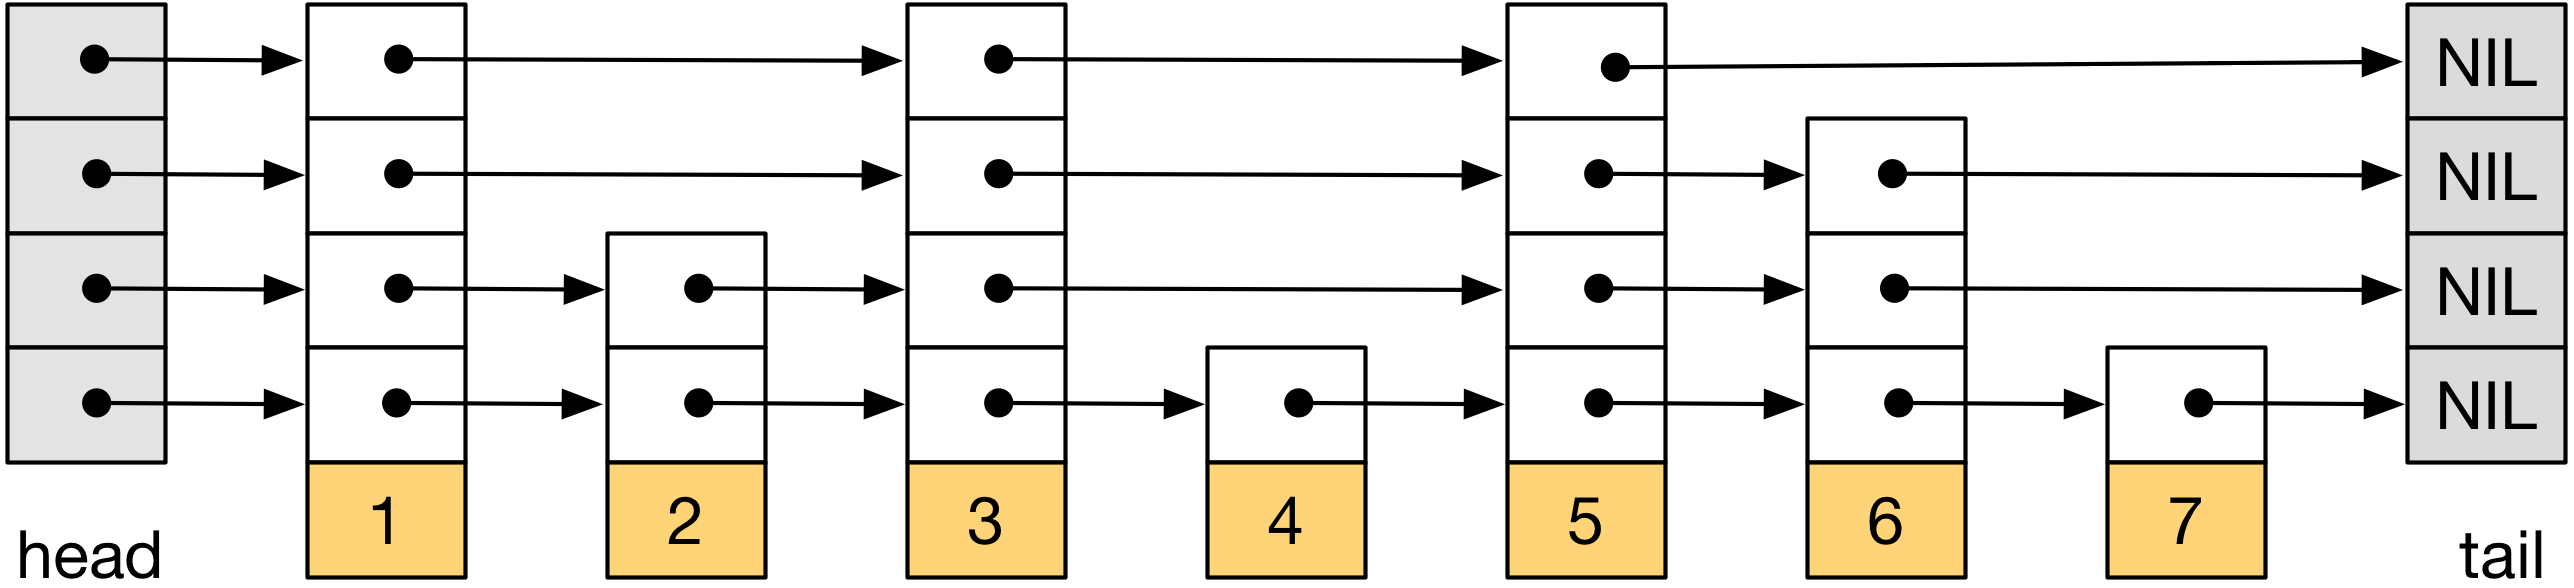
\includegraphics[scale=0.4]{images/fig-2}
\caption{Skiplist}
\label{fig:skiplist}
\end{figure}
Skiplist is a probabilistic balanced ordered search data structure \cite{pugh:skiplist}. We could describe skiplist as a group of sorted singly linked lists arranged in levels to facilitate the binary search. The lowest level (level 0) is a singly linked list of nodes that hold data. The upper levels of the skiplist work as the index into the lower levels. Each level in the skiplist has approximately n/f nodes, where n is the number nodes in the next lower level. The fanout factor, f determines the multiplication factor of index nodes in the skiplist. This constant factor can be tuned for allowing the tradeoff between memory and CPU usage. Each node in the skiplist has a level which is assigned probabilistically. For a level 3 skiplist node, there will be three forward node pointers. Theoretically, skiplists consume only 1.33 forward pointers per node.

Skiplist supports operations for insert, lookup, and delete with an average case complexity of O(log(n)). Skiplist lookup algorithm is similar to the binary search on a sorted array. For example, to find a node with key 4 from the Skiplist in the Figure 1, the search starts from the level 4 (top level) head node and checks if the node pointed by the forward pointer has a key less than 4. If so, move to the next node on the same level. Repeat until a node with a key greater than or equal to key 4 is found. When a node with a greater or equal key is encountered (key 5 in this example), search level is decremented by 1. This is repeated until level 0 is reached. A sequential search is performed in the level 0 linked list. In this example, level 0 is reached with a node with key 3. The next node in the level 0 is the node with key 4. The lookup algorithm can be extended to implement insert and delete. 

The skiplist operations can be modified by proper usage of atomic instructions to make them thread-safe and avoid any usage of locks for synchronization. The techniques for implementing Insert and Delete operations for lock-free skiplist are discussed by Sundell and Tsigas \cite{lockfree-skiplist} and a simplified variant in book, \textit{The Art of Multiprocessor Programming} \cite{art-of-multproc}. The lock-free insert and delete operations on the skiplist involve two phases. The first phase for the insert involves adding the new node into the level 0 (data level) linked list. During the second phase, the new node is linked to all the upper levels (index levels) linked lists. Similarly, the first phase of delete involves unlinking the node from all the upper levels (index levels) and during second phase node is unlinked from level 0 (data level). The first and second phase do not require any synchronization. This is an important property of skiplist that facilitates easier implementation of lock-free operations.

The lock-free operations for skiplist are implemented on the basis of lock-free linked list algorithms \cite{valois:lockfree-list}. The atomic \textit{CompareAndSwap (CAS)} operation is used to make sure that no two threads modify the same next node pointer. If multiple threads are trying to update the same next pointer, only one thread succeeds and others fail. Failed threads have to restart the operation by restarting the algorithm.

\begin{figure}[H]
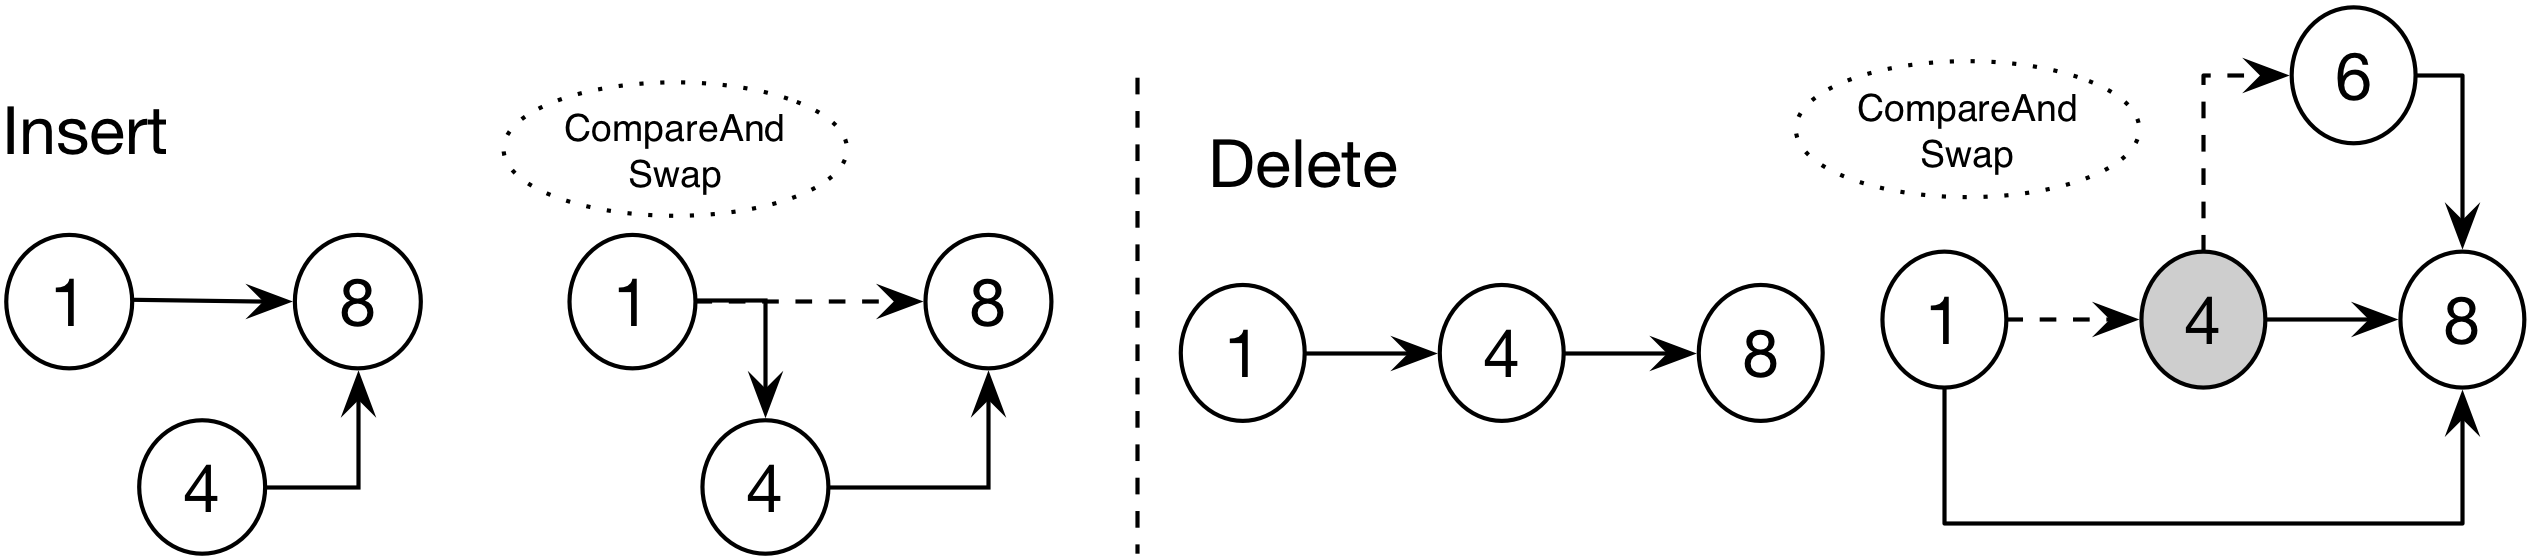
\includegraphics[scale=0.4]{images/fig-3}
\caption{Lockfree list insert/delete operations}
\label{fig:lockfree-list}
\end{figure}

The example in Figure 2 illustrates lock-free insert and delete algorithms for a linked list. The insertion into a linked list is straightforward using CAS. But the delete operation is more involved when multiple threads operate concurrently. Let us consider a case with two threads A and B operating concurrently. Thread A is trying to delete node 4 by performing a CAS on the next pointer of the node 1. Thread B is trying to insert a node 6 between node 4 and node 8. It is possible that both Thread A and Thread B succeeds their operations since the two threads are performing CAS on two different pointers belonging to different nodes. The insertion operation of node 6 can succeed while its predecessor node has been removed. Even though the insert operation for node 6 has succeeded, it will not appear in the skiplist leading to incorrectness.

When the insert for node 6 is processed by updating the predecessor and the predecessor node is currently being deleted, the operation should fail in order to ensure correctness. A two-step delete approach can be used to perform the safe delete by adding an atomically markable flag to the pointer. First, the \textit{next} pointer of the node that needs to be deleted is atomically marked as deleted. In the second step, the \textit{next} pointer of the predecessor node is atomically swapped with a pointer to the next node. An insert operation on the node being deleted would fail since the predecessor node's \textit{next} pointer is marked as deleted. This mark flag demands additional flag to be compared atomically during CAS operation. That is, a pair of pointer and flag needs to be compared using a \textit{DoubleCAS} operation. Instead of using \textit{CAS(prev\_next, new\_next)}, now we need to use \textit{DoubleCAS([prev\_next, prev\_isdeleted], [new\_next, new\_isdeleted])}. \textit{DoubleCAS} instruction is not available on all hardware platforms.

We used a different approach to achieve \textit{DoubleCAS} without any hardware support. Instead of next pointers, we defined a new object type for pointer next reference. The reference object holds two values, a node pointer and a \textit{isdeleted} mark flag. Instead of doing CompareAndSwap on the node pointer, we perform CompareAndSwap on a pointer to this next reference object. Thus, every time the reference object is swapped, two values are atomically swapped. For a non-garbage collected language, other approaches such as tagged pointers can be used. The least 48 bits of the 64-bit virtual addresses are only used in practice. The MSB bit of the 64-bit pointer address can be used to indicate \textit{isdeleted} flag. This tagging method can avoid the extra memory overhead of pointer reference object.


In addition to the insert, delete and lookup operations, we required the ability to do skiplist iterations for range queries. We implemented capability for lock-free skiplist iteration. To traverse a range of nodes in the skiplist, the start node is located using lookup operation. The subsequent seek to the next nodes are performed by atomically loading next node pointer. If the next pointer has its \textit{isdeleted} flag marked, the iterator has to stop and refresh the next pointer by doing a lookup to the current item and continue. Iterator also implements co-operative delete of nodes if it encounters a node with \textit{next} pointer marked as deleted.

\section{Nitro MVCC Design}
The multi-version concurrency control system is the core of Nitro. We implement multi-version concurrency control as a layer on top of the lock-free skiplist. The MVCC system provides the transactional properties for the lock-free skiplist.

We designed MVCC layer to provide following features:

\textbf{Immutable snapshots:} Concurrent writers add or remove items into the skiplist. A snapshot of the current items can be created to provide a point-in-time view of the skiplist. This is useful for providing repeatable stable scans. Users can create and manage multiple snapshots. If an application requires atomicity for a batch of skiplist operations, it can apply a batch of operations and create a new snapshot. Changes would be invisible until a new snapshot is created.

\textbf{Fast and low overhead snapshots:} Readers of the skiplist use a snapshot handle to perform all lookup and range queries. An indexer application typically requires many snapshots to be created every second for servicing index queries. So the overhead of creating and maintaining a snapshot should be minimal for servicing the high rate of snapshot generation. Nitro snapshots are very cheap and is an O(1) operation.


\textbf{Avoid phantom reads:} A query operation using a snapshot will always return the same results. Items being removed or added will not be visible to the query. A query operation using a snapshot is repeatable.


\textbf{Memory efficiency:} Disk oriented data structures such as append only copy-on-write B+Tree process updates in the unit of disk page sizes \cite{couchdb}. This approach introduces significant storage overhead per item. For a single entry update, the entire residing page needs to be copied. Nitro allocates the only exact amount of space required to hold an item. This is also important for predictable capacity planning.

\textbf{Fast and scalable garbage collection:} For a system that generates hundred immutable snapshots per second, there could be a hundred snapshots becoming unused every second. MVCC Garbage collector should be efficient enough to keep up with higher rates of garbage generation. Nitro garbage collector is concurrent and scales with the number of concurrent writers used by the system.

\subsection{Structural modifications}
In this section, we describe how multi-version based \textit{Insert}, \textit{Delete}, \textit{CreateSnapshot}, \textit{DeleteSnapshot} functionalities are implemented.


Once an item is added into the MVCC skiplist, it becomes immutable. If an item needs to be updated, the previous node for the item is marked as deleted and a new node is inserted. Thus, multiple versions of the same item key can exist in the MVCC skiplist. If two versions of the same key exist, the latest version is considered as a higher value than the previous version according to the Nitro's skiplist sort order. For implementing the MVCC system, we add a metadata attribute to every node in the skiplist. We call this node metadata, \textit{lifetime}. Lifetime is denoted using a tuple (\textit{bornSn, deadSn}). We call it born snapshot number and dead snapshot number. The storage engine maintains a current snapshot number, \textit{termSn} for the database. The \textit{termSn} is incremented during every snapshot create operation. These three primitives are used to implement all the MVCC operations. 

 \begin{figure}[H]
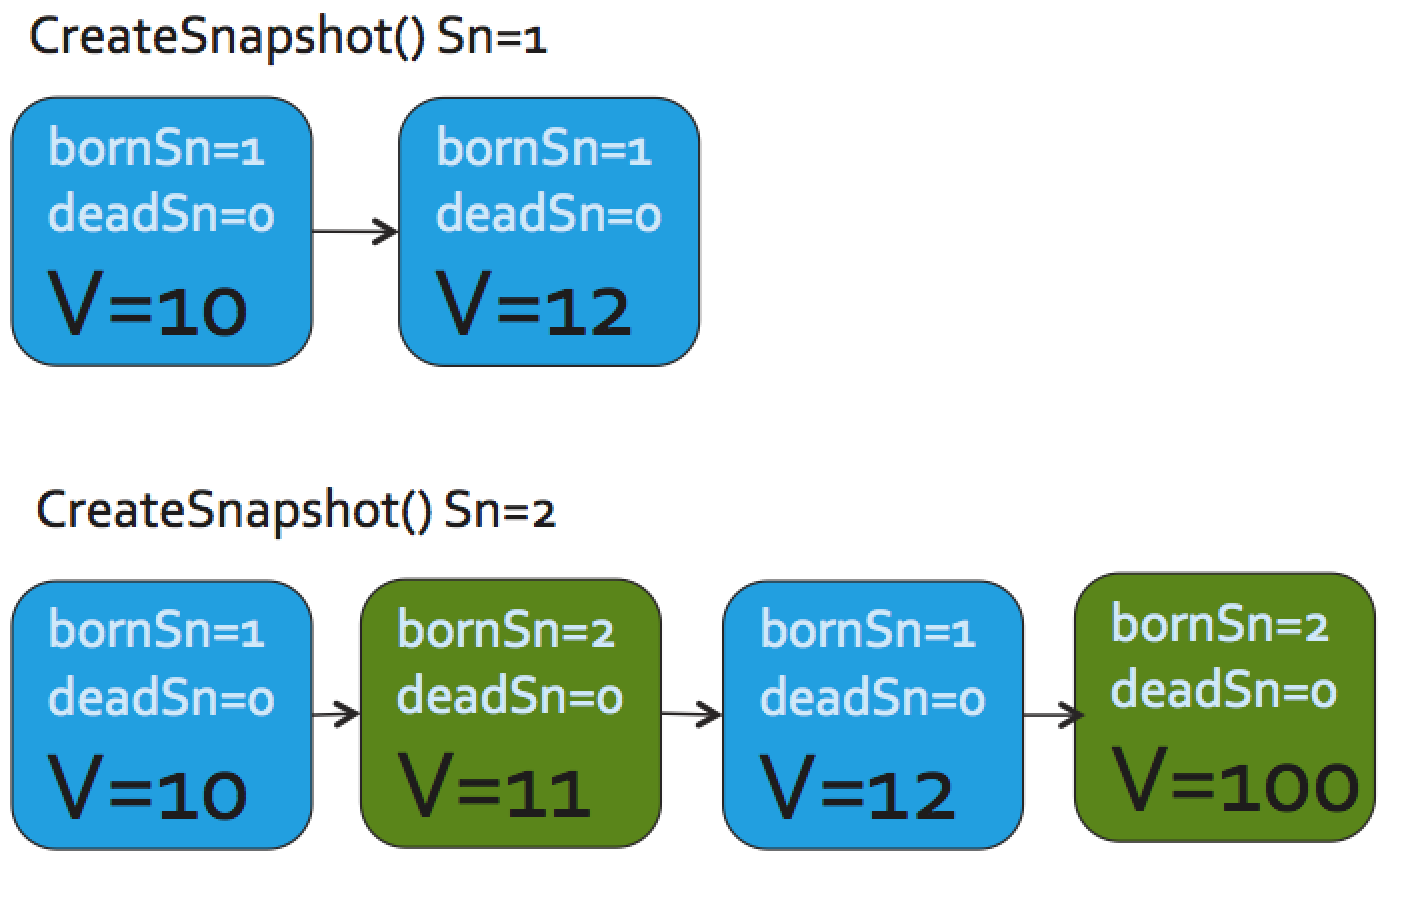
\includegraphics[scale=0.5]{images/fig-4}
\caption{Snapshotting based on versions of items}
\label{fig:mvcc}
\end{figure}

The storage engine initially starts with \textit{termSn=1}. When a node is inserted into the skiplist, the \textit{bornSn} of the node is set to the current snapshot number, \textit{termSn} and \textit{deadSn} to 0. The zero value of the \textit{deadSn} denotes that the node is never marked as dead. The skiplist uses a key comparator that additionally considers the \textit{bornSn} for determining the sort order. If there are two items in the skiplist with same key, it will consider \textit{bornSn} to decide the sort order. When an item needs to be deleted, a skiplist lookup is performed and sets \textit{deadSn} as the current \textit{termSn} for the node to be deleted. The node is not immediately removed from the skiplist. Unlinking of the node is performed by the garbage collector as it becomes unused by all the consumers in the system. The \textit{bornSn} and \textit{deadSn} are immutable once they are set. Given a \textit{termSn}, we can easily answer the question whether an item is valid with respect to a \textit{termSn} by looking at the \textit{bornSn} and \textit{deadSn}.

An immutable snapshot is created by atomically incrementing the global \textit{termSn} by 1. Creating a snapshot is an O(1) operation and hence very inexpensive. A snapshot descriptor representing the snapshot is allocated as part of snapshot creation.  Snapshot descriptor manages reference counting for the snapshot accessors. Consumers of the immutable snapshot (e.g., index application scan requests), increments the reference count of the snapshot and decrements the reference count once it has finished using the snapshot. Once the reference count for a snapshot becomes zero, the snapshot is eligible for deletion and the garbage collector can be notified to remove the dead nodes from the snapshot. The memory consumption for maintaining a snapshot is minimal. Memory required for maintaining a snapshot is equal to the number of items in a snapshot and few bytes of snapshot metadata. This makes the Nitro MVCC system a good fit for an in-memory index use case.

Items belonging to different snapshots co-exist in the same skiplist ordered by (\textit{key, bornSn}). As an optimization, if \textit{bornSn} and \textit{deadSn} are same as the current \textit{termSn}, we immediately unlink the node from the skiplist rather than waiting for the garbage collector as the item is invisible until an immutable snapshot is created. The Figure 3 shows level 0 nodes of the lock-free linked list in the sorted order. Each node has an MVCC \textit{lifetime} metadata attached to it.
    
\subsection{Snapshot Iteration}
The MVCC skiplist snapshot iterator is built on top of the lock-free skiplist iterator. The MVCC snapshot iterator is aware of the \textit{bornSn} and \textit{deadSn} lifetime metadata of the skiplist nodes. A snapshot iterator is created from a snapshot descriptor. An iterator initialization operation increments the snapshot reference count to prevent the snapshot from getting garbage collected while iteration operation is in progress. An iterator is associated with the snapshot number (\textit{termSn}) obtained from the snapshot descriptor. Iterator implements \textit{SeekFirst()}, \textit{Seek()}, \textit{Next()}, \textit{Valid()} APIs. When \textit{Next()} is called, it obtains the next node in the skiplist and evaluates whether the items are visible with respect to the iterator \textit{termSn}. The iterator will filter all the items in the skiplist with \textit{bornSn} $>$ \textit{termSn} and \textit{deadSn} $\geq$ \textit{termSn}. Even though many versions of the items are visited during the lock-free skiplist iteration, the MVCC skiplist iterator returns only the necessary items which are alive with respect to the snapshot \textit{termSn}. The complexity of item lookup in the skiplist is O(log(n)). Every subsequent sequential seek to the next item has an amortized complexity of O(1). The MVCC skiplist snapshot iterator can be used to implement operations such as key lookup and range queries. 


 \begin{figure}[h]
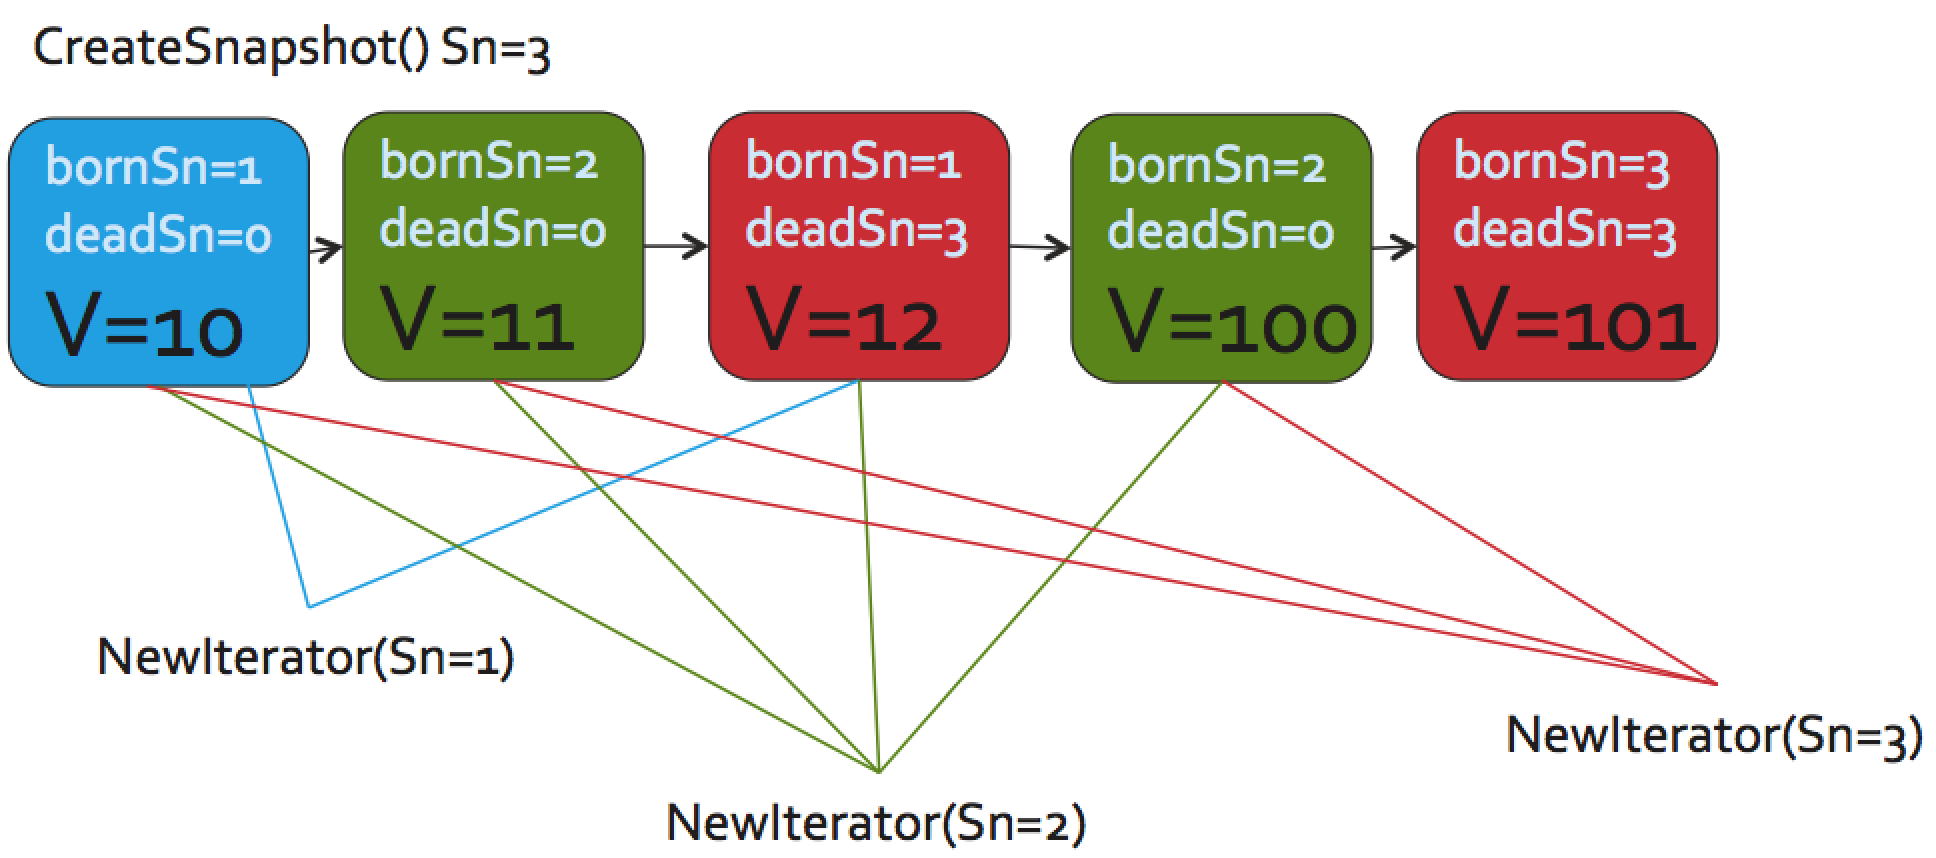
\includegraphics[scale=0.45]{images/fig-5}
\caption{Iterator operation on a snapshot}
\label{fig:snap-iterator}
\end{figure}

The Figure 4 illustrates the visibility of items in the skiplist for different iterators assigned with Sn=1, Sn=2, and Sn=3.
An iterator with Sn=1 will only observe items V=10 and V=12. Since others were born after the \textit{termSn=1}, they are hidden by the iterator.

 An iterator with Sn=2 will observe nodes with V=10, V=11, V=12 and V=100. An iterator with Sn=3 will not observe items with V=12 and V=101 as they are marked as dead during \textit{termSn=3}.

\subsection{Comparison with Copy-On-Write B+Tree}
Disk-oriented storage systems like CouchDB \cite{couchdb}, Btrfs \cite{btrfs} use append-only Copy-On-Write (COW) B+tree as the core data structure for storage. They inherently support multi-versioning and snapshotting. We evaluated this approach while designing our in-memory storage engine. Copy-on-write append only B+Tree operates in the chunks of pages and it requires periodic compaction operations to remove stale blocks and keep the storage used under control. Typically, they assume that 2x storage is available. Memory is a limited resource and we wanted to reduce memory usage as much as possible.

The concurrent structural modification operations on a B+Tree requires serialization of access to the B+Tree pages and it is very difficult to achieve parallelism. Coarse-grained data access in B+Tree may require many latches for concurrent operation implementation. Scaling with many cores with B+Tree is a difficult problem.


 \begin{figure}[H]
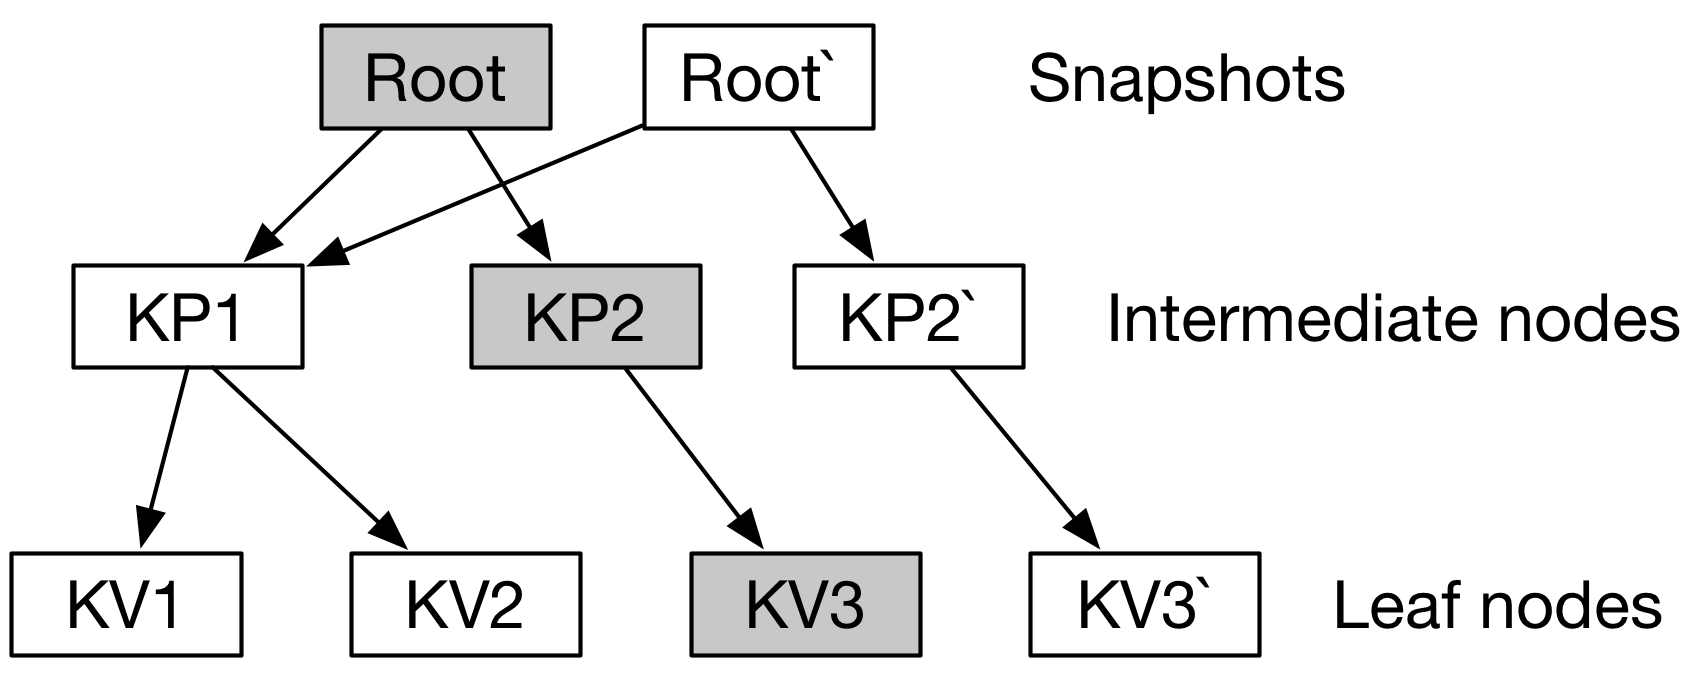
\includegraphics[scale=0.5]{images/fig-6}
\caption{Copy-on-write B+Tree snapshot}
\label{fig:btree-cow}
\end{figure}

Copy-On-Write append only B+Trees have very high storage requirement for keeping multiple snapshots alive as the data is only stored in leaf nodes and they have intermediate nodes. Any modification operation of an item has to touch at least a page block. A single item insert may require copying of  $log_B (n)$ pages. As shown in the diagram, if an item is modified or added into KV3, it has to copy a leaf node (KV3), an intermediate node (KP2) and root node (Root). This is extremely inefficient for an in-memory system. 

It is a common technique to amortize the storage requirement by accumulating insert and delete operations in a batch and perform a bulk update. This may cause the commit operation to stall for a long time. In an application where hundreds of snapshots are generated per second, we expect few dozens of live snapshots at any point in time and efficiency of creating snapshots is the key to throughput, latency, and predictability of the system. These characteristics are not acceptable in a write-heavy in-memory storage system which needs to scale with a number of cores.

\section{Garbage Collection}
In an MVCC system, a high-performance garbage collector is required for the cleaning stale objects and to keep the memory usage under control. A write-heavy application can create hundreds of snapshots per second. The applications manage the snapshots being used by incrementing the reference count of the snapshot descriptor. When the application decides that a snapshot is no longer required, it decrements the reference count. When a snapshot's reference count becomes zero, the dead items or deleted items in that snapshot are eligible for unlinking from the skiplist.


During each snapshot term, items are getting inserted and few other items are getting marked as deleted. A skiplist node is qualified for garbage collection if nobody is interested in reading from snapshots with \textit{termSn} less than the \textit{deadSn} of the node. As you know that nodes in the skiplist are immutable, every update results in marking an old node as deleted and the addition of a new node. This can generate multiple versions of the same item in the skiplist. The Nitro delete operation succeeds by logically deleting an item by setting \textit{deadSn} field in the skiplist node. Keeping many logically deleted nodes in the skiplist for longer duration can cause performance degradation. They hold up additional memory and increase the memory footprint of the system. All the items are linked in level 0 linked list of the skiplist. If there are many deleted items in the list, an iterator traversing the skiplist may have to unnecessarily go through many stale nodes and skip them. The cost of sequential seeks can exceed O(1).

Whenever a snapshot's reference count becomes zero, it is not sufficient to trigger garbage collection of that snapshot. Each snapshot Sn(x), is dependent on the snapshot Sn(x-1). Consider an example of \textit{termSn=1} where itemX and itemY were inserted. In a snapshot with \textit{termSn=2}, itemX was deleted. Assume that snapshot with \textit{termSn=1} is currently being used by an application. But the snapshot with \textit{termSn=2} is unused and its reference count becomes zero. If we decide to remove items which are marked as deleted in \textit{termSn=2}, we would end up removing itemX. But the \textit{termSn=1} is being used an application and it may notice missing of itemX while performing a range query or iteration. This will break the scan stability property offered by the Nitro snapshots. Garbage collection of snapshots can only be performed in the sequential order of the snapshot \textit{termSn}. This condition has to be met before garbage collecting a snapshot.

A simple approach for implementing garbage collection is to dedicate a thread that traverses the entire skiplist and performs removal of the nodes from the skiplist. Periodically the least unreferenced \textit{termSn} can be determined and collector thread can remove the nodes with \textit{deadSn} $\leq$ least unused \textit{termSn}. But, the single thread approach is not scalable. Depending on the workload, may be only a few percent of the skiplist items are being modified while other items remain the same. Scanning the entire skiplist for finding the small percent of dead nodes is inefficient. The storage engine supports many concurrent writers in the lock-free skiplist. Each writer can delete items from skiplist independently. A single thread for garbage collection can never keep up with the rate of garbage generated by the multiple writers. We need garbage collection workers equal to the number of writer workers. 

Nitro supports concurrent writers for inserting or removing items in the skiplist. Each writer maintains a \textit{deadList} data structure to help the garbage collector. Whenever a node is marked as deleted by a Nitro writer, the marked node is added into the \textit{deadList}. Thus, each writer has a list of skiplist nodes marked as deleted. Whenever the application invokes \textit{CreateSnapshot()} API, it collects the local lists from each of the writers and stitches them together. This global list has reference to all the skiplist nodes which are marked as deleted during the snapshot period. This \textit{deadList} is attached to the snapshot descriptor. As part of a snapshot garbage collection, garbage collection workers uses this \textit{deadList} of a snapshot to perform physical node removal from the skiplist.
    

\section{Backup and Recovery}
The durability of data is important for any storage system. As Nitro keeps all data in memory, backing up data on disk enables it to recover from crashes or application restarts using local data. Nitro is optimized for indexes disjoint from main document store and assumes indexes can be rebuilt from older persisted snapshots. Nitro supports creating a backup on disk from a given snapshot. If an application can create a snapshot periodically at consistent checkpoints, they can be used for creating backups on disk. The recovery mechanism reads the backup files and reconstructs the immutable snapshot. We have designed Nitro backup and recovery to be concurrent and scalable with the available CPU cores.


\subsection{Backing up snapshot to Disk}
A disk backup can be created from a Nitro snapshot. A Nitro backup is the dump of items in a snapshot to a set of files. The idea is to traverse level 0 linked list of the lock-free skiplist and write out the entries into data files. During this traversal, all the entries not belonging to the given snapshot are ignored. A simple binary data file format with a length prefix for the item is used for backup files. We do not store any node \textit{lifetime} metadata in the backup files as they can be recreated during recovery. As the items in the level 0 linked list of the skiplist are sort ordered, the data written on the disk is also ordered in nature. The disk space requirement for the snapshot file is exactly equal to the total size of items and an additional two bytes per item for storing item length. This simple format can also make the best use of data compression. Since the items are sort ordered, compression algorithms can reduce the size of backup files significantly. Compression will require additional CPU cycles to be spent. But, a fast data compression library such as snappy can be used for reducing the storage required for the backups. Backup involves sequential writes to the disk, which is known to be beneficial for both Hard Disk (HDD) and Solid State Devices (SSD).

A backup task is started by incrementing the reference count for the snapshot descriptor and the reference count is decremented once the backup task has finished. This is to prevent the snapshot from being garbage collected during the backup traversal. The downside of the backup process is that it can eventually halt the garbage collector until the backup task is finished.

Linked lists are cache unfriendly due to poor spatial locality. Traversing the level 0 linked list can be time-consuming for a large skiplist. During the backup period, memory usage can increase due to pausing of the garbage collector in order to prevent nodes from getting garbage collected. We implemented a concurrent visitor for the lock-free skiplist. The visitor is able to run worker threads equal to the number of cores. If there are a number of skiplist instances in the system, we assign workers proportional to the number of items in each skiplist. If a skiplist has n items and k workers, each worker has to scan approximately n/k items. This is only possible if each worker is provided with start node of n/kth segments in the skiplist. Reaching n/k(i) th element in the skiplist requires traversing O(n) items and it is impractical. We used a different approach to approximately determine n/k(i) nodes. Since we have used fanout factor for the skiplist as 4, every level in the skiplist has approximately n/4 nodes, where n is the number of nodes in the next lower level. If there are four nodes at level 3, that means each of them approximately divides the skiplist into four segments. We maintain a skiplist statistics about the number of nodes in each level. Based on this information, we can find out the level with at least k nodes. This statistics can be used to split the level 0 list into k range partitions. These range partition information is used to locate start and end nodes for each of the workers. We also shard the data files for the backups based on these range partitions which helps to utilize parallel channels found on modern SSDs. Sharded files also facilitate to apply parallel rebuild algorithms during recovery. As the disk writes are efficient when large blocks are used, backup flusher workers accumulate records in larger chunks for each batch of write.
       
\subsection{Recovering from Disk Backup}
During index recovery, we spawn concurrent worker threads equal to the number of backup shard files.
Each worker associated with a backup shard file performs restore operation for the items from its file. The simple approach for rebuilding the skiplist is to concurrently perform skiplist insert operation for the items read from each file. This approach is inefficient since the concurrent writers may observe CompareAndSwap conflicts and need to repeat the insert operation by spending many CPU cycles. Disk-oriented databases with B+Tree as underlying data structure commonly uses bulk loading technique to build an efficient B+Tree bottom-up from a large set of sorted items. We use a similar approach for recovering Nitro from backup.

As the backup shard files are partitioned by sort ordered ranges, they are well suited for reconstructing the skiplist using the concurrent bottom-up build technique. The idea of the skiplist bottom-up build is to construct the sorted level 0 singly linked list and simultaneously add higher levels of linked lists in the skiplist. During the addition of each item, the level of that node is determined probabilistically. A temporary level buffer array, \textit{Buf[MaxLevel]} is used to store previous node pointers in each level. Initially node pointers for all levels are set to nil in \textit{Buf}. When a node at level x is added, \textit{Buf} array indexes 0 to x-1 are updated with a pointer to the current node. The next pointers of the previous nodes stored by \textit{Buf} array indexes 0 to x-1 are set to the new node. Entire skiplist can be build at a complexity of O(n).

Let us walk through an example of how we could build the skiplist in the Figure 1. \textit{Buf[0-3]} is set to nil. Now, a node 1 with probabilistically determined level 4 needs to be added. \textit{Buf[0-3]} is set to a pointer to the node 1. Next, we need to add node 2 at level 2. So the next pointer of nodes pointed by \textit{Buf[0-1]} (node 1) are set to node 2. \textit{Buf[0-1]} are updated with pointers to the node 2. To add node 3 with level 4, the next pointer of nodes in \textit{Buf[0-4]} are set to node 3, i.e., second and third level next pointer of node 1 points to node 3 and the zero and first level next pointers of node 2 points to node 3. Similarly, the entire skiplist can be build.

 The skiplist bottom-up build algorithm can be concurrently executed by having each worker thread that builds skiplist segment for a shard file. Once all the workers have finished building skiplist segments, all the segments can be stitched together to form the global skiplist. Shard files are named appropriately to keep the sort order by its minimum item key. Next pointers of the tail nodes from each skiplist segment can be set to point to the head nodes of next skiplist segment as per the shard file order. Once the build is complete, a new snapshot descriptor representing the restored snapshot is created. In this method, the skiplist segment builds can proceed without any synchronization and scales linearly with the number of cores.


\subsection{Non-intrusive backup}
The regular backup algorithm has the disadvantage that it needs to hold the snapshot to prevent it from getting garbage collected until the backup is complete. This would eventually halt garbage collection happening during the backup if it takes longer to complete. The non-intrusive backup facilitates to perform the backup operation without halting the garbage collection operation and it can operate in the background without increasing the memory usage.

When a backup operation is in-progress, items in the backup snapshot may get marked as deleted due to the latest modifications happening in the skiplist. When the garbage collection runs, it unlinks those items from the skiplist if the snapshot refcount is 0 and the backup task may miss items from the snapshot. However, the backup task will never observe any new items outside of the snapshot. The key idea of the non-intrusive backup is to collect the possible missing items in the backup with the help of garbage collector to reconstruct the backup snapshot. The items in the backup snapshot would be the union of partial snapshot items observed by the backup task and the items which were removed by the garbage collector. The delta of deleted items can be obtained from the garbage collector workers since they are responsible for physical removal of nodes from the skiplist. 


When a backup task is started, it sets the state to INIT and notifies garbage collection workers that it is going to start backup on snapshot \textit{termSn}. Garbage collection workers acknowledge the notification, copies \textit{termSn} to its local config and initializes per-worker delta backup files. Backup task moves to ACTIVE state and initializes concurrent flushers for writing delta files. During ACTIVE state, garbage collection workers check if a node belongs to the backup \textit{termSn} by comparing \textit{bornSn} and \textit{deadSn} before performing unlink from the skiplist and eligible items are written into the corresponding delta data file. Once the main backup task finishes scanning the skiplist, it moves to TERMINATING state and waits for garbage collector workers to acknowledge. Garbage collection workers close the delta file, clears the backup \textit{termSn} and backup task finishes its operation. Now we have two set of data files. The first set of files containing unique sort ordered items written by backup task and the second set of files containing the set of items possibly missed by the main backup task. Delta files may contain duplicate items which could be present in main data files. This method of backup is non-intrusive as the Nitro garbage collector can operate without pausing. Delta file writers use append-only write pattern which is efficient for SSDs and disks.

During the recovery, the snapshot restore task needs to process these delta files. Recovery happens in two phases. The first phase involves concurrent bottom-up skiplist rebuild from the main backup files. During the second phase, concurrent delta restore worker threads equal to the number of delta files are started. Each worker reads items from the delta file sequentially and performs insertion into the skiplist. The delta insert operations can fail if the same items exist in the skiplist as they were restored from the main backup files during the first phase.

The tradeoff for this method is that the delta files can contain the duplicate items which are already written by main backup task and may require extra disk storage space. The extra storage requirement can be estimated based on the expected rate of delete operations. Since the delta files have unordered items, they cannot be populated into the skiplist using bottom-up build method. The time for recovery can be higher since it executes an additional delta recovery phase.

\section{Safe memory reclamation}
The MVCC model for lock-free skiplist described in the earlier section facilitates to remove nodes from the skiplist belonging to a snapshot once they become unused. Removal of the node only involves unlinking the node from the skiplist. The freeing of the node cannot be performed immediately since there could be active threads such as iterators may be holding valid references to an unlinked node. While lock-free data structure provides high performance and scalability, the reclamation of removed nodes from the data structure becomes complex due to  a number of threads independently accessing the nodes in the data structures concurrently without any synchronization. When a node is removed, we cannot free the node immediately since we do not know if a thread is still referencing the node \cite{hp,ebr}. If we decide to reuse a node after unlinking from the lock-free data structure, it may lead to nasty bugs and incorrectness. Applications using garbage collected programming languages can usually avoid this concern since the language runtime takes care of safe reclamation. Reference counting every node is the simplest approach for solving this problem where blocking synchronization can be used and it is expensive. Our initial implementation depends on Golang's mark and sweep garbage collector for safe reclamation. But, testing showed unacceptable performance and lack of predictable memory usage. We describe a novel algorithm for safe memory reclamation for Nitro to overcome the limitations of language runtime based safe reclamation.

We implement a safe memory reclamation technique taking advantage of our MVCC system. We wanted an SMR system that performs very well without causing any performance degradation for Nitro. The algorithm builds on few simple ideas and assumptions. The safety conditions for Nitro reclamation are as follows:

\begin{enumerate}
  \item Any thread accessing the lock-free skiplist is called an accessor.
  \item If there are no accessors currently present in the skiplist for a node unlinked from the skiplist, it is safe to free the node.
  \item If a node n is unlinked at a time, t0. Any accessors that came after t0 will not be able to access the node n or hold a reference to node n.
  \item If there are k accessors in the skiplist after a node n is unlinked, from (3) we know that it is safe to free node n once k accessors finish their operation.
  \item If x nodes are unlinked, it is safe to unlink these x nodes once all the accessors which were present in the skiplist during xth node unlink leave the skiplist.
\end{enumerate}

We introduced few abstractions in our system for easy implementation of safe reclamation algorithm.

\textbf{AccessBarrier:} Nitro skiplist has a global data structure called AccessBarrier that controls access to the skiplist.
 Any thread requiring access to the skiplist needs to be passed through a gate which tracks the safety conditions for freeing nodes. Accessor needs to acquire an access token from the access barrier. Once the thread has finished operation on the skiplist, it has to release the access token. An access barrier holds a reference to barrier session object.

\textbf{BarrierSession:} Barrier session tracks the number of live accessors currently operating on the skiplist. AccessBarrier holds the latest barrier session. Barrier session object holds a 32 bit counter called liveCount, which is initialized to zero.

\textbf{BarrierSessionClose:} When a barrier session close is invoked, current barrier session is made immutable. No more accessor will be added to the current barrier session. AccessBarrier will initialize a new barrier session. A barrier session is said to be terminated when all the accessors in the barrier session finish the operation.


In this algorithm, the unit of safety period is a barrier session. All the live accessors of the skiplist are tracked in a barrier session. Whenever a skiplist delete or group of deletes are performed, current barrier session is closed and a new barrier session is started. The closed barrier is responsible for safe reclamation of deleted node(s). The closed barrier session has a record of all accessors belonging to that session. The right time to safely reclaim the node(s) is when all the accessors become dead. This makes sure that unlinked nodes will be invisible to any new accessors. The accessors in the barrier session can co-operatively detect and mark when each of them terminates. When the last accessor in a barrier session terminates, it can take the action to call the destructor for the node(s).


\subsection{Accessor operation}
When an accessor enters the skiplist, it acquires an access token which is a reference to barrier session held by the access barrier. As part of returning access token, liveCount is atomically incremented by 1. When the accessor leaves the skiplist, liveCount in the token is atomically decremented by 1. When a node removal or group of deletes are performed, BarrierSessionClose is initialized. BarrierSessionClose atomically swaps the access barrier's BarrierSession with a new empty session. Thus, any further incoming accessors would mark them in the new session. The old session becomes immutable and no new accessor would add itself to the closed session. There could be race conditions causing accessors to accidentally add them to the closed session soon after a session is closed. We have a detect and recover mechanism to unregister accessor by itself from the barrier session. We will describe the details in the next section.

\subsection{BarrierSessionClose operation}
After a node is removed from the skiplist, immediately barrier session close is initiated. As part of the session close, it notes down the list of nodes to be freed. We assume that a maximum number of accessors in a session is always less than MaxInt32/2. During session close, an offset MaxInt32/2 is atomically added to the liveCount of the current session. A liveCount greater than or equal to MaxInt32/2 indicates that the session is closed. Now, the current barrier session in the access barrier is swapped with a new barrier session. All the accessors accidentally entering the barrier session can detect if it is a closed session by checking the return value of atomic increment of liveCount to see if it is greater than MaxInt32/2. Otherwise, it will atomically decrement and retry to register them for the new session. Once all the accessors of the session finish operation, liveCount is decremented and finally it becomes MaxInt32/2. The last leaving accessor can execute the freeing of nodes, which were noted down during the barrier session close initialization.


\subsection{Garbage collector integration}
Every Nitro operation such as Insert, Delete and Iteration goes through the access barrier. We have dedicated SMR free worker threads equal to the number of garbage collection workers. The garbage collector processes the skiplist nodes removal in the batches of \textit{deadList} from the snapshots. Each dead snapshot has a \textit{deadList}. When a garbage collector worker finishes processing a dead snapshot, it initializes a barrier session close with snapshot's unlinked nodes list. Once the barrier session becomes terminated, it invokes session destructor by passing the \textit{deadList} of nodes. The registered destructor hands off the \textit{deadList} to one of the free workers. The free worker is responsible for executing node freeing for all the nodes in the received list.

\subsection{Long running iterators}
Index iterators can be running for a longer period of time since they are often used for large range queries or full dataset scan. For example, during snapshot backup to disks, an iterator is going to live for a long time. That means it will take a long time for a barrier session to get terminated. Unless they are terminated, nodes are not going to be freed and it can increase the memory usage by the indexer. We solve this problem by refreshing iterators periodically. When an iterator traverses a certain number of items, we close the current iterator and reopen the iterator from the offset node where it left off. This would make sure that iterator accessor is not holding a barrier session by preventing its termination for too long.

\section{Nitro Performance}
The focus of our performance evaluation is to showcase the throughput scalability of Insert and Get operations.

\textbf{Setup:} The performance tests have been conducted on a machine having Intel(R) Xeon(R) CPU E5-2650 v3 2.30GHz with 40 virtual cores and 128 GB of DRAM. We installed Debian Linux 7 on this node. We used randomly generated small keys of size 8 bytes to 128 bytes for the tests. The skiplist was populated with a total of 20 million items in each of the tests.
\begin{figure}[h]
% GNUPLOT: LaTeX picture with Postscript
\begingroup
  \makeatletter
  \providecommand\color[2][]{%
    \GenericError{(gnuplot) \space\space\space\@spaces}{%
      Package color not loaded in conjunction with
      terminal option `colourtext'%
    }{See the gnuplot documentation for explanation.%
    }{Either use 'blacktext' in gnuplot or load the package
      color.sty in LaTeX.}%
    \renewcommand\color[2][]{}%
  }%
  \providecommand\includegraphics[2][]{%
    \GenericError{(gnuplot) \space\space\space\@spaces}{%
      Package graphicx or graphics not loaded%
    }{See the gnuplot documentation for explanation.%
    }{The gnuplot epslatex terminal needs graphicx.sty or graphics.sty.}%
    \renewcommand\includegraphics[2][]{}%
  }%
  \providecommand\rotatebox[2]{#2}%
  \@ifundefined{ifGPcolor}{%
    \newif\ifGPcolor
    \GPcolorfalse
  }{}%
  \@ifundefined{ifGPblacktext}{%
    \newif\ifGPblacktext
    \GPblacktexttrue
  }{}%
  % define a \g@addto@macro without @ in the name:
  \let\gplgaddtomacro\g@addto@macro
  % define empty templates for all commands taking text:
  \gdef\gplbacktext{}%
  \gdef\gplfronttext{}%
  \makeatother
  \ifGPblacktext
    % no textcolor at all
    \def\colorrgb#1{}%
    \def\colorgray#1{}%
  \else
    % gray or color?
    \ifGPcolor
      \def\colorrgb#1{\color[rgb]{#1}}%
      \def\colorgray#1{\color[gray]{#1}}%
      \expandafter\def\csname LTw\endcsname{\color{white}}%
      \expandafter\def\csname LTb\endcsname{\color{black}}%
      \expandafter\def\csname LTa\endcsname{\color{black}}%
      \expandafter\def\csname LT0\endcsname{\color[rgb]{1,0,0}}%
      \expandafter\def\csname LT1\endcsname{\color[rgb]{0,1,0}}%
      \expandafter\def\csname LT2\endcsname{\color[rgb]{0,0,1}}%
      \expandafter\def\csname LT3\endcsname{\color[rgb]{1,0,1}}%
      \expandafter\def\csname LT4\endcsname{\color[rgb]{0,1,1}}%
      \expandafter\def\csname LT5\endcsname{\color[rgb]{1,1,0}}%
      \expandafter\def\csname LT6\endcsname{\color[rgb]{0,0,0}}%
      \expandafter\def\csname LT7\endcsname{\color[rgb]{1,0.3,0}}%
      \expandafter\def\csname LT8\endcsname{\color[rgb]{0.5,0.5,0.5}}%
    \else
      % gray
      \def\colorrgb#1{\color{black}}%
      \def\colorgray#1{\color[gray]{#1}}%
      \expandafter\def\csname LTw\endcsname{\color{white}}%
      \expandafter\def\csname LTb\endcsname{\color{black}}%
      \expandafter\def\csname LTa\endcsname{\color{black}}%
      \expandafter\def\csname LT0\endcsname{\color{black}}%
      \expandafter\def\csname LT1\endcsname{\color{black}}%
      \expandafter\def\csname LT2\endcsname{\color{black}}%
      \expandafter\def\csname LT3\endcsname{\color{black}}%
      \expandafter\def\csname LT4\endcsname{\color{black}}%
      \expandafter\def\csname LT5\endcsname{\color{black}}%
      \expandafter\def\csname LT6\endcsname{\color{black}}%
      \expandafter\def\csname LT7\endcsname{\color{black}}%
      \expandafter\def\csname LT8\endcsname{\color{black}}%
    \fi
  \fi
    \setlength{\unitlength}{0.0500bp}%
    \ifx\gptboxheight\undefined%
      \newlength{\gptboxheight}%
      \newlength{\gptboxwidth}%
      \newsavebox{\gptboxtext}%
    \fi%
    \setlength{\fboxrule}{0.5pt}%
    \setlength{\fboxsep}{1pt}%
\begin{picture}(5040.00,3772.00)%
    \gplgaddtomacro\gplbacktext{%
      \csname LTb\endcsname%
      \put(1078,704){\makebox(0,0)[r]{\strut{}$0$}}%
      \put(1078,984){\makebox(0,0)[r]{\strut{}$5000$}}%
      \put(1078,1265){\makebox(0,0)[r]{\strut{}$10000$}}%
      \put(1078,1545){\makebox(0,0)[r]{\strut{}$15000$}}%
      \put(1078,1825){\makebox(0,0)[r]{\strut{}$20000$}}%
      \put(1078,2106){\makebox(0,0)[r]{\strut{}$25000$}}%
      \put(1078,2386){\makebox(0,0)[r]{\strut{}$30000$}}%
      \put(1078,2666){\makebox(0,0)[r]{\strut{}$35000$}}%
      \put(1078,2946){\makebox(0,0)[r]{\strut{}$40000$}}%
      \put(1078,3227){\makebox(0,0)[r]{\strut{}$45000$}}%
      \put(1078,3507){\makebox(0,0)[r]{\strut{}$50000$}}%
      \put(1210,484){\makebox(0,0){\strut{}$0$}}%
      \put(1782,484){\makebox(0,0){\strut{}$5\times10^{7}$}}%
      \put(2354,484){\makebox(0,0){\strut{}$1\times10^{8}$}}%
      \put(2927,484){\makebox(0,0){\strut{}$1.5\times10^{8}$}}%
      \put(3499,484){\makebox(0,0){\strut{}$2\times10^{8}$}}%
      \put(4071,484){\makebox(0,0){\strut{}$2.5\times10^{8}$}}%
      \put(4643,484){\makebox(0,0){\strut{}$3\times10^{8}$}}%
    }%
    \gplgaddtomacro\gplfronttext{%
      \csname LTb\endcsname%
      \put(176,2105){\rotatebox{-270}{\makebox(0,0){\strut{}Time taken}}}%
      \put(2926,154){\makebox(0,0){\strut{}Number of items}}%
      \csname LTb\endcsname%
      \put(3656,1097){\makebox(0,0)[r]{\strut{}Backup}}%
      \csname LTb\endcsname%
      \put(3656,877){\makebox(0,0)[r]{\strut{}Recovery}}%
    }%
    \gplbacktext
    \put(0,0){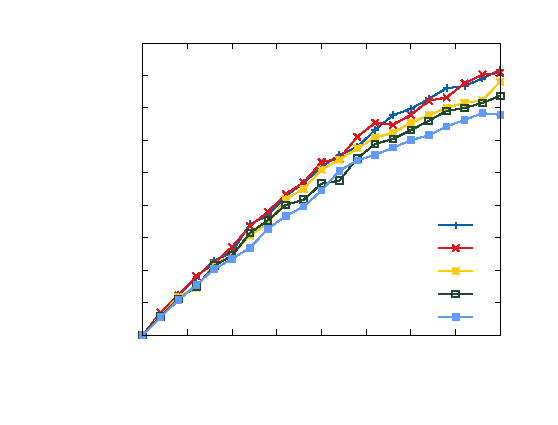
\includegraphics{insert_scale_plot}}%
    \gplfronttext
  \end{picture}%
\endgroup

\caption{Insert throughput}
\label{fig:throughput-threads}
\end{figure}

\begin{figure}[h]
% GNUPLOT: LaTeX picture with Postscript
\begingroup
  \makeatletter
  \providecommand\color[2][]{%
    \GenericError{(gnuplot) \space\space\space\@spaces}{%
      Package color not loaded in conjunction with
      terminal option `colourtext'%
    }{See the gnuplot documentation for explanation.%
    }{Either use 'blacktext' in gnuplot or load the package
      color.sty in LaTeX.}%
    \renewcommand\color[2][]{}%
  }%
  \providecommand\includegraphics[2][]{%
    \GenericError{(gnuplot) \space\space\space\@spaces}{%
      Package graphicx or graphics not loaded%
    }{See the gnuplot documentation for explanation.%
    }{The gnuplot epslatex terminal needs graphicx.sty or graphics.sty.}%
    \renewcommand\includegraphics[2][]{}%
  }%
  \providecommand\rotatebox[2]{#2}%
  \@ifundefined{ifGPcolor}{%
    \newif\ifGPcolor
    \GPcolorfalse
  }{}%
  \@ifundefined{ifGPblacktext}{%
    \newif\ifGPblacktext
    \GPblacktexttrue
  }{}%
  % define a \g@addto@macro without @ in the name:
  \let\gplgaddtomacro\g@addto@macro
  % define empty templates for all commands taking text:
  \gdef\gplbacktext{}%
  \gdef\gplfronttext{}%
  \makeatother
  \ifGPblacktext
    % no textcolor at all
    \def\colorrgb#1{}%
    \def\colorgray#1{}%
  \else
    % gray or color?
    \ifGPcolor
      \def\colorrgb#1{\color[rgb]{#1}}%
      \def\colorgray#1{\color[gray]{#1}}%
      \expandafter\def\csname LTw\endcsname{\color{white}}%
      \expandafter\def\csname LTb\endcsname{\color{black}}%
      \expandafter\def\csname LTa\endcsname{\color{black}}%
      \expandafter\def\csname LT0\endcsname{\color[rgb]{1,0,0}}%
      \expandafter\def\csname LT1\endcsname{\color[rgb]{0,1,0}}%
      \expandafter\def\csname LT2\endcsname{\color[rgb]{0,0,1}}%
      \expandafter\def\csname LT3\endcsname{\color[rgb]{1,0,1}}%
      \expandafter\def\csname LT4\endcsname{\color[rgb]{0,1,1}}%
      \expandafter\def\csname LT5\endcsname{\color[rgb]{1,1,0}}%
      \expandafter\def\csname LT6\endcsname{\color[rgb]{0,0,0}}%
      \expandafter\def\csname LT7\endcsname{\color[rgb]{1,0.3,0}}%
      \expandafter\def\csname LT8\endcsname{\color[rgb]{0.5,0.5,0.5}}%
    \else
      % gray
      \def\colorrgb#1{\color{black}}%
      \def\colorgray#1{\color[gray]{#1}}%
      \expandafter\def\csname LTw\endcsname{\color{white}}%
      \expandafter\def\csname LTb\endcsname{\color{black}}%
      \expandafter\def\csname LTa\endcsname{\color{black}}%
      \expandafter\def\csname LT0\endcsname{\color{black}}%
      \expandafter\def\csname LT1\endcsname{\color{black}}%
      \expandafter\def\csname LT2\endcsname{\color{black}}%
      \expandafter\def\csname LT3\endcsname{\color{black}}%
      \expandafter\def\csname LT4\endcsname{\color{black}}%
      \expandafter\def\csname LT5\endcsname{\color{black}}%
      \expandafter\def\csname LT6\endcsname{\color{black}}%
      \expandafter\def\csname LT7\endcsname{\color{black}}%
      \expandafter\def\csname LT8\endcsname{\color{black}}%
    \fi
  \fi
    \setlength{\unitlength}{0.0500bp}%
    \ifx\gptboxheight\undefined%
      \newlength{\gptboxheight}%
      \newlength{\gptboxwidth}%
      \newsavebox{\gptboxtext}%
    \fi%
    \setlength{\fboxrule}{0.5pt}%
    \setlength{\fboxsep}{1pt}%
\begin{picture}(5040.00,3772.00)%
    \gplgaddtomacro\gplbacktext{%
      \csname LTb\endcsname%
      \put(946,704){\makebox(0,0)[r]{\strut{}0  }}%
      \put(946,984){\makebox(0,0)[r]{\strut{}1 M}}%
      \put(946,1265){\makebox(0,0)[r]{\strut{}2 M}}%
      \put(946,1545){\makebox(0,0)[r]{\strut{}3 M}}%
      \put(946,1825){\makebox(0,0)[r]{\strut{}4 M}}%
      \put(946,2106){\makebox(0,0)[r]{\strut{}5 M}}%
      \put(946,2386){\makebox(0,0)[r]{\strut{}6 M}}%
      \put(946,2666){\makebox(0,0)[r]{\strut{}7 M}}%
      \put(946,2946){\makebox(0,0)[r]{\strut{}8 M}}%
      \put(946,3227){\makebox(0,0)[r]{\strut{}9 M}}%
      \put(946,3507){\makebox(0,0)[r]{\strut{}10 M}}%
      \put(1078,484){\makebox(0,0){\strut{}$0$}}%
      \put(1524,484){\makebox(0,0){\strut{}$5$}}%
      \put(1969,484){\makebox(0,0){\strut{}$10$}}%
      \put(2415,484){\makebox(0,0){\strut{}$15$}}%
      \put(2861,484){\makebox(0,0){\strut{}$20$}}%
      \put(3306,484){\makebox(0,0){\strut{}$25$}}%
      \put(3752,484){\makebox(0,0){\strut{}$30$}}%
      \put(4197,484){\makebox(0,0){\strut{}$35$}}%
      \put(4643,484){\makebox(0,0){\strut{}$40$}}%
    }%
    \gplgaddtomacro\gplfronttext{%
      \csname LTb\endcsname%
      \put(176,2105){\rotatebox{-270}{\makebox(0,0){\strut{}Throughput (items/s)}}}%
      \put(2860,154){\makebox(0,0){\strut{}Number of cores}}%
      \csname LTb\endcsname%
      \put(3920,1757){\makebox(0,0)[r]{\strut{}Get 8 bytes}}%
      \csname LTb\endcsname%
      \put(3920,1537){\makebox(0,0)[r]{\strut{}Get 16 bytes}}%
      \csname LTb\endcsname%
      \put(3920,1317){\makebox(0,0)[r]{\strut{}Get 32 bytes}}%
      \csname LTb\endcsname%
      \put(3920,1097){\makebox(0,0)[r]{\strut{}Get 64 bytes}}%
      \csname LTb\endcsname%
      \put(3920,877){\makebox(0,0)[r]{\strut{}Get 128 bytes}}%
    }%
    \gplbacktext
    \put(0,0){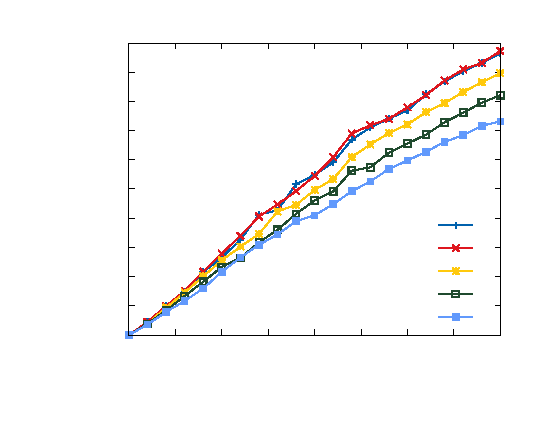
\includegraphics{get_scale_plot}}%
    \gplfronttext
  \end{picture}%
\endgroup

\caption{Get throughput}
\label{fig:throughput-threads}
\end{figure}

 \begin{figure}[h]
% GNUPLOT: LaTeX picture with Postscript
\begingroup
  \makeatletter
  \providecommand\color[2][]{%
    \GenericError{(gnuplot) \space\space\space\@spaces}{%
      Package color not loaded in conjunction with
      terminal option `colourtext'%
    }{See the gnuplot documentation for explanation.%
    }{Either use 'blacktext' in gnuplot or load the package
      color.sty in LaTeX.}%
    \renewcommand\color[2][]{}%
  }%
  \providecommand\includegraphics[2][]{%
    \GenericError{(gnuplot) \space\space\space\@spaces}{%
      Package graphicx or graphics not loaded%
    }{See the gnuplot documentation for explanation.%
    }{The gnuplot epslatex terminal needs graphicx.sty or graphics.sty.}%
    \renewcommand\includegraphics[2][]{}%
  }%
  \providecommand\rotatebox[2]{#2}%
  \@ifundefined{ifGPcolor}{%
    \newif\ifGPcolor
    \GPcolorfalse
  }{}%
  \@ifundefined{ifGPblacktext}{%
    \newif\ifGPblacktext
    \GPblacktexttrue
  }{}%
  % define a \g@addto@macro without @ in the name:
  \let\gplgaddtomacro\g@addto@macro
  % define empty templates for all commands taking text:
  \gdef\gplbacktext{}%
  \gdef\gplfronttext{}%
  \makeatother
  \ifGPblacktext
    % no textcolor at all
    \def\colorrgb#1{}%
    \def\colorgray#1{}%
  \else
    % gray or color?
    \ifGPcolor
      \def\colorrgb#1{\color[rgb]{#1}}%
      \def\colorgray#1{\color[gray]{#1}}%
      \expandafter\def\csname LTw\endcsname{\color{white}}%
      \expandafter\def\csname LTb\endcsname{\color{black}}%
      \expandafter\def\csname LTa\endcsname{\color{black}}%
      \expandafter\def\csname LT0\endcsname{\color[rgb]{1,0,0}}%
      \expandafter\def\csname LT1\endcsname{\color[rgb]{0,1,0}}%
      \expandafter\def\csname LT2\endcsname{\color[rgb]{0,0,1}}%
      \expandafter\def\csname LT3\endcsname{\color[rgb]{1,0,1}}%
      \expandafter\def\csname LT4\endcsname{\color[rgb]{0,1,1}}%
      \expandafter\def\csname LT5\endcsname{\color[rgb]{1,1,0}}%
      \expandafter\def\csname LT6\endcsname{\color[rgb]{0,0,0}}%
      \expandafter\def\csname LT7\endcsname{\color[rgb]{1,0.3,0}}%
      \expandafter\def\csname LT8\endcsname{\color[rgb]{0.5,0.5,0.5}}%
    \else
      % gray
      \def\colorrgb#1{\color{black}}%
      \def\colorgray#1{\color[gray]{#1}}%
      \expandafter\def\csname LTw\endcsname{\color{white}}%
      \expandafter\def\csname LTb\endcsname{\color{black}}%
      \expandafter\def\csname LTa\endcsname{\color{black}}%
      \expandafter\def\csname LT0\endcsname{\color{black}}%
      \expandafter\def\csname LT1\endcsname{\color{black}}%
      \expandafter\def\csname LT2\endcsname{\color{black}}%
      \expandafter\def\csname LT3\endcsname{\color{black}}%
      \expandafter\def\csname LT4\endcsname{\color{black}}%
      \expandafter\def\csname LT5\endcsname{\color{black}}%
      \expandafter\def\csname LT6\endcsname{\color{black}}%
      \expandafter\def\csname LT7\endcsname{\color{black}}%
      \expandafter\def\csname LT8\endcsname{\color{black}}%
    \fi
  \fi
    \setlength{\unitlength}{0.0500bp}%
    \ifx\gptboxheight\undefined%
      \newlength{\gptboxheight}%
      \newlength{\gptboxwidth}%
      \newsavebox{\gptboxtext}%
    \fi%
    \setlength{\fboxrule}{0.5pt}%
    \setlength{\fboxsep}{1pt}%
\begin{picture}(5040.00,3772.00)%
    \gplgaddtomacro\gplbacktext{%
      \csname LTb\endcsname%
      \put(946,704){\makebox(0,0)[r]{\strut{}0  }}%
      \put(946,984){\makebox(0,0)[r]{\strut{}1 M}}%
      \put(946,1265){\makebox(0,0)[r]{\strut{}2 M}}%
      \put(946,1545){\makebox(0,0)[r]{\strut{}3 M}}%
      \put(946,1825){\makebox(0,0)[r]{\strut{}4 M}}%
      \put(946,2106){\makebox(0,0)[r]{\strut{}5 M}}%
      \put(946,2386){\makebox(0,0)[r]{\strut{}6 M}}%
      \put(946,2666){\makebox(0,0)[r]{\strut{}7 M}}%
      \put(946,2946){\makebox(0,0)[r]{\strut{}8 M}}%
      \put(946,3227){\makebox(0,0)[r]{\strut{}9 M}}%
      \put(946,3507){\makebox(0,0)[r]{\strut{}10 M}}%
      \put(1078,484){\makebox(0,0){\strut{}$0$}}%
      \put(1524,484){\makebox(0,0){\strut{}$5$}}%
      \put(1969,484){\makebox(0,0){\strut{}$10$}}%
      \put(2415,484){\makebox(0,0){\strut{}$15$}}%
      \put(2861,484){\makebox(0,0){\strut{}$20$}}%
      \put(3306,484){\makebox(0,0){\strut{}$25$}}%
      \put(3752,484){\makebox(0,0){\strut{}$30$}}%
      \put(4197,484){\makebox(0,0){\strut{}$35$}}%
      \put(4643,484){\makebox(0,0){\strut{}$40$}}%
    }%
    \gplgaddtomacro\gplfronttext{%
      \csname LTb\endcsname%
      \put(176,2105){\rotatebox{-270}{\makebox(0,0){\strut{}Throughput (items/s)}}}%
      \put(2860,154){\makebox(0,0){\strut{}Number of cores}}%
      \csname LTb\endcsname%
      \put(4052,1097){\makebox(0,0)[r]{\strut{}Get 16 bytes}}%
      \csname LTb\endcsname%
      \put(4052,877){\makebox(0,0)[r]{\strut{}Get with background inserts}}%
    }%
    \gplbacktext
    \put(0,0){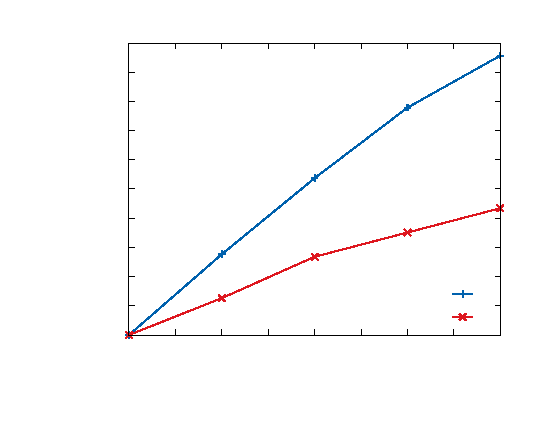
\includegraphics{getbg_scale_plot}}%
    \gplfronttext
  \end{picture}%
\endgroup

\caption{Get with mutations throughput}
\label{fig:throughput-threads}
\end{figure}

\begin{figure}[h]
% GNUPLOT: LaTeX picture with Postscript
\begingroup
  \makeatletter
  \providecommand\color[2][]{%
    \GenericError{(gnuplot) \space\space\space\@spaces}{%
      Package color not loaded in conjunction with
      terminal option `colourtext'%
    }{See the gnuplot documentation for explanation.%
    }{Either use 'blacktext' in gnuplot or load the package
      color.sty in LaTeX.}%
    \renewcommand\color[2][]{}%
  }%
  \providecommand\includegraphics[2][]{%
    \GenericError{(gnuplot) \space\space\space\@spaces}{%
      Package graphicx or graphics not loaded%
    }{See the gnuplot documentation for explanation.%
    }{The gnuplot epslatex terminal needs graphicx.sty or graphics.sty.}%
    \renewcommand\includegraphics[2][]{}%
  }%
  \providecommand\rotatebox[2]{#2}%
  \@ifundefined{ifGPcolor}{%
    \newif\ifGPcolor
    \GPcolorfalse
  }{}%
  \@ifundefined{ifGPblacktext}{%
    \newif\ifGPblacktext
    \GPblacktexttrue
  }{}%
  % define a \g@addto@macro without @ in the name:
  \let\gplgaddtomacro\g@addto@macro
  % define empty templates for all commands taking text:
  \gdef\gplbacktext{}%
  \gdef\gplfronttext{}%
  \makeatother
  \ifGPblacktext
    % no textcolor at all
    \def\colorrgb#1{}%
    \def\colorgray#1{}%
  \else
    % gray or color?
    \ifGPcolor
      \def\colorrgb#1{\color[rgb]{#1}}%
      \def\colorgray#1{\color[gray]{#1}}%
      \expandafter\def\csname LTw\endcsname{\color{white}}%
      \expandafter\def\csname LTb\endcsname{\color{black}}%
      \expandafter\def\csname LTa\endcsname{\color{black}}%
      \expandafter\def\csname LT0\endcsname{\color[rgb]{1,0,0}}%
      \expandafter\def\csname LT1\endcsname{\color[rgb]{0,1,0}}%
      \expandafter\def\csname LT2\endcsname{\color[rgb]{0,0,1}}%
      \expandafter\def\csname LT3\endcsname{\color[rgb]{1,0,1}}%
      \expandafter\def\csname LT4\endcsname{\color[rgb]{0,1,1}}%
      \expandafter\def\csname LT5\endcsname{\color[rgb]{1,1,0}}%
      \expandafter\def\csname LT6\endcsname{\color[rgb]{0,0,0}}%
      \expandafter\def\csname LT7\endcsname{\color[rgb]{1,0.3,0}}%
      \expandafter\def\csname LT8\endcsname{\color[rgb]{0.5,0.5,0.5}}%
    \else
      % gray
      \def\colorrgb#1{\color{black}}%
      \def\colorgray#1{\color[gray]{#1}}%
      \expandafter\def\csname LTw\endcsname{\color{white}}%
      \expandafter\def\csname LTb\endcsname{\color{black}}%
      \expandafter\def\csname LTa\endcsname{\color{black}}%
      \expandafter\def\csname LT0\endcsname{\color{black}}%
      \expandafter\def\csname LT1\endcsname{\color{black}}%
      \expandafter\def\csname LT2\endcsname{\color{black}}%
      \expandafter\def\csname LT3\endcsname{\color{black}}%
      \expandafter\def\csname LT4\endcsname{\color{black}}%
      \expandafter\def\csname LT5\endcsname{\color{black}}%
      \expandafter\def\csname LT6\endcsname{\color{black}}%
      \expandafter\def\csname LT7\endcsname{\color{black}}%
      \expandafter\def\csname LT8\endcsname{\color{black}}%
    \fi
  \fi
    \setlength{\unitlength}{0.0500bp}%
    \ifx\gptboxheight\undefined%
      \newlength{\gptboxheight}%
      \newlength{\gptboxwidth}%
      \newsavebox{\gptboxtext}%
    \fi%
    \setlength{\fboxrule}{0.5pt}%
    \setlength{\fboxsep}{1pt}%
\begin{picture}(5040.00,3772.00)%
    \gplgaddtomacro\gplbacktext{%
      \csname LTb\endcsname%
      \put(814,704){\makebox(0,0)[r]{\strut{}1 M}}%
      \put(814,1104){\makebox(0,0)[r]{\strut{}2 M}}%
      \put(814,1505){\makebox(0,0)[r]{\strut{}3 M}}%
      \put(814,1905){\makebox(0,0)[r]{\strut{}4 M}}%
      \put(814,2306){\makebox(0,0)[r]{\strut{}5 M}}%
      \put(814,2706){\makebox(0,0)[r]{\strut{}6 M}}%
      \put(814,3107){\makebox(0,0)[r]{\strut{}7 M}}%
      \put(814,3507){\makebox(0,0)[r]{\strut{}8 M}}%
      \put(946,484){\makebox(0,0){\strut{}1}}%
      \put(2178,484){\makebox(0,0){\strut{}2}}%
      \put(3411,484){\makebox(0,0){\strut{}3}}%
      \put(4643,484){\makebox(0,0){\strut{}4}}%
    }%
    \gplgaddtomacro\gplfronttext{%
      \csname LTb\endcsname%
      \put(176,2105){\rotatebox{-270}{\makebox(0,0){\strut{}Throughput (items/s)}}}%
      \put(2794,154){\makebox(0,0){\strut{}Number of Partitions}}%
      \csname LTb\endcsname%
      \put(4052,877){\makebox(0,0)[r]{\strut{}Insert 16 bytes items/sec}}%
    }%
    \gplbacktext
    \put(0,0){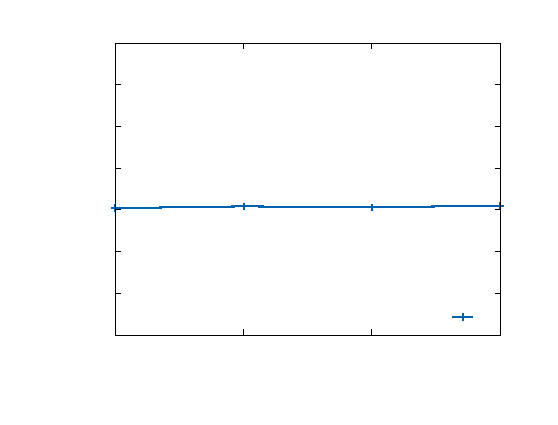
\includegraphics{part_plot}}%
    \gplfronttext
  \end{picture}%
\endgroup

\caption{Scaling with number of partitions}
\label{fig:throughput-threads}
\end{figure}


\textbf{Experiment 1:} We ran a test against a Nitro instance with varying number of insert workers. Each worker was responsible for populating an equal number of items. Fixed size keys were generated randomly by each of the workers. We repeated the experiment with different key sizes from 8 bytes to 128 bytes. In Figure 6, we show that the insert throughput is linearly scalable with the number of cores used. We observed that the throughput per core remains approximately 100,000 items/sec. A maximum insertion throughput of 4 million inserts/sec was observed with 40 cores.

\textbf{Experiment 2:} In this experiment, we evaluated the scalability of lookup operations. Similar to the Experiment 1, we used a varying number of lookup workers for the test. Each lookup worker performed an equal number of lookups.
The Figure 7 shows a maximum throughput of 10 million lookups/sec with 40 cores and the lookup throughput scales linearly.


\textbf{Experiment 3:} In a real world workload, it is common to have both insert and lookup operations happening concurrently against a datastore. We ran a test to evaluate the effect of background inserts on the lookup throughput. The test was conducted with an equal number of insert and lookup workers operating on a 20M items skiplist. Figure 8 shows the pattern of throughput scaling for this test.


\textbf{Experiment 4:} Partitioning is a common approach to scale performance. If the throughput of a data structure does not scale with a single instance, multiple instances can be used and workload can be sharded between the instances. We evaluated whether Nitro shows any improvement in insertion throughput by varying the number of Nitro instances. The Figure 9 shows that the data structure does not require any partitioning to improve performance. Partitioned instances of Nitro delivers almost the same throughput as a single instance with 40 cores.

\textbf{Memory requirements:} The predictable memory requirements of Nitro storage engine makes it easier for applications to calculate memory usage. The approximate memory usage for an item inserted into the skiplist is 64 bytes + itemSize bytes. The memory used by the multiple live snapshots is (64 + AvgitemSize)*numberOfLiveSnapshots.

\textbf{Observations:} In all of the above throughput tests, Nitro saturated all 40 CPU cores. The CPU profiling shows that the CPU was mostly spent in atomic load and compare-and-swap operations. Therefore, we are not able to saturate the available memory bandwidth.

\section{Couchbase GSI Overview}
 \begin{figure}[h]
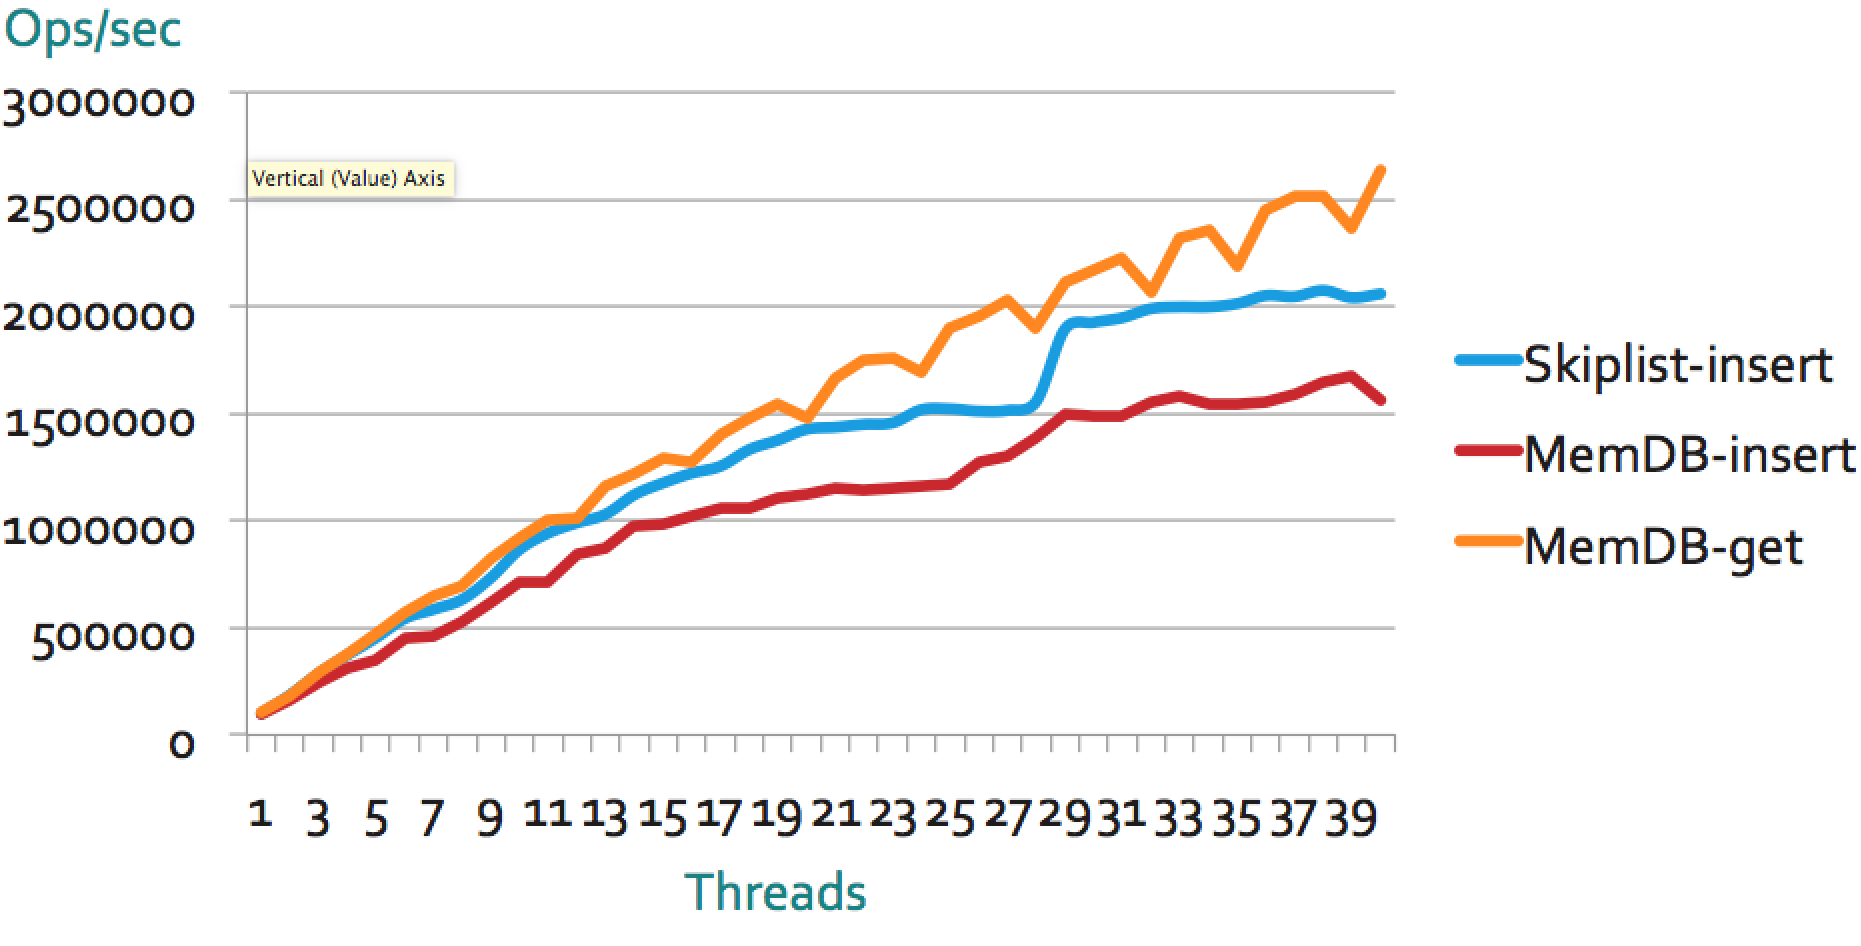
\includegraphics[scale=0.45]{images/fig-7}
\caption{GSI architecture}
\label{fig:mvcc}
\end{figure}
Couchbase is a high performance distributed NoSQL document database. Couchbase uses JSON as the document format and it supports creating secondary indexes on JSON fields. Couchbase leverages scale-out architecture and has the ability to independently scale different set of services on a separate group of server nodes. We call the document storage system of Couchbase as Data Service and index storage system as Index Service \cite{mds}.

The data service uniformly distributes the documents to many nodes by hashing on the primary key of the document in order to ensure that resource consumption is balanced throughout the cluster. For a local secondary index, it is impossible to scan a range of records/documents from the index using a secondary key without having to visit every single node in the cluster. Local secondary indexes are often designed to be updated synchronously during the primary key update. If there are a number of secondary indexes, it can eventually affect the throughput of the primary key update. To design a scale-out secondary index, the index needs to be partitioned independently from the primary key. Couchbase Global Secondary Index (GSI) is designed by considering these aspects.

The independent placing of indexes on a separate set of nodes introduces few challenges. The indexes are updated asynchronously with respect to the data services. The preferred deployment model for GSI indexes is to host many indexes on a single large node. This avoids the needs for contacting multiple index nodes for performing index scan. As index node receives document changes from many data services nodes and it has to maintain many indexes, the single index performance matters. If there are 5 data service nodes in the cluster, and each of the nodes receives documents at a rate x, the index node will receive documents at a rate 5x. A high-performance index storage engine is required to keep up with the high mutation rate. The documents are sent over to the index nodes via the network protocol called Database Change Protocol (DCP) \cite{dcp}.

\subsection{Index update operations} 
The GSI index engine needs to maintain two data structures for its operation. An index data structure and a lookup data structure. The index data structure stores the secondary key index and is used by index scans. The lookup data structure, called as \textit{reverse-map} is a supporting data structure for index update operations. We will walk through the sequence of index engine operations to understand these data structures in detail.

Consider an example of secondary indexing on JSON documents. A document with a primary key, "employee-1" has a JSON body \{"id"€: 1022, €"city"€: "€œBangalore"€, "title"€: "€œSoftware Engineer"€\}. If a secondary index is created on the field "€œcity"€, an index scan can be performed by specifying a range on "city". For the above document, the city-index will have an entry \{key: "€œBangalore"€, primary: "€œemployee-1"€\}. If the document is updated by changing the city from "Bangalore" to "€œMountainView"€,  the corresponding city-index entry should be updated as \{key:"€œMountainView"€, primary: "€œemployee-1"€\}. That means we need to delete the previous index entry for the primary key, "employee-1" before inserting the new index entry. For that, we should be able to retrieve the previous secondary index entry for a given primary key. We maintain a \textit{reverse-map} data structure for this purpose. It maps primary key to the current secondary index entry. The index update pipeline performs the following operations for every document. First, the \textit{reverse-map} is queried to see if an entry exists. If it exists, we remove that entry from the index and an insert of new entry into the index is performed. Finally, the \textit{reverse-map} data structure is updated with mapping to the new index entry.

The index engine periodically creates snapshots of the index for serving scan operation. A query can read items only using an index snapshot. The index snapshot interval affects the latency of consistent index queries since indexes are updated asynchronously with respect to the primary document.

\subsection{Index service recovery}
Documents in the Couchbase data service are hash partitioned into a fixed set of hash buckets. Document changes are processed sequentially for each hash bucket. Each document update is assigned an incrementing sequence number per hash bucket. The set of sequence numbers for all the buckets forms a vector clock. When the index update engine periodically creates index snapshots, this vector clock is stored as metadata of the snapshot. When an indexer crash occurs, a recently persisted index snapshot is recovered by using the underlying storage engine. The \textit{reverse-map} data structure also needs to be recovered. The indexer reads the vector clock from the snapshot metadata and requests the data service to restart the mutation stream from the given vector clock. The data service is capable of restarting the document changes stream from the given sequence numbers for each hash bucket. When an index is created for the first time, it requests data service with a zero vector clock value.

\section{Nitro Integration for GSI}
In this section, we look at how we integrated Nitro into the GSI index engine for Memory Optimized Index (MOI). The primary goal of using Nitro for GSI was to make use of all the CPU cores and deliver index operations with high throughput with low latency. We had to make our index update pipeline tuned for concurrency to push maximum operations into Nitro. Using Nitro as the core index data structure also helps us significantly reduce storage requirement and CPU cycles required for maintaining the \textit{reverse-map} data structure.

\textbf{Partitioning:} If the index update throughput has to scale with a number of cores, we need to parallelize index updates operations and distribute load uniformly across each core. We used a partitioning approach for index update pipeline. Simple round-robin partitioning can break the sequential order of document updates and can cause the index to become inconsistent. For example, two operations \{delete, docid\} and \{insert, docid, key\} can arrive into the index update pipeline. If we decide to evenly distribute them among two concurrent worker threads, \{delete, docid\} and \{insert, docid, key\} operations can occur in any order. If the \{insert, docid, key\} operation was applied before \{delete, docid\}, this can lead to incorrectness. According to the correct order, a delete should occur before an insert. So, we need to ensure that ordering of document updates for a document primary key is always preserved. Out-of-order execution of operations for documents with different primary key will not cause such incorrectness as Couchbase operations are document scoped. We implemented partitioning using the CRC32 hash of the document primary key to ensure that the upstream mutation order is preserved.

\textbf{Optimizations for reverse-map data structure:} The index pipeline has concurrent index update worker threads equal to the number of cores. For index pipeline to be concurrent, both index data structure and \textit{reverse-map} data structure should support thread-safe concurrent access. The straightforward solution is to use Nitro for the index as well as \textit{reverse-map} data structure. A similar approach has been used in Couchbase 4.0 with regular indexes. We used the same B+Tree based storage engine for index and \textit{reverse-map}. The purpose of \textit{reverse-map} data structure is to retrieve the current index entry corresponding to a primary key, so that the previous entry can be removed before inserting a new index entry. The \textit{reverse-map} data structure is only used in the update pipeline and so it does not require snapshotting capability. As we have partitioned documents uniformly into index update worker threads, a document with the same primary key will uniquely map to one of the worker threads. This property helps to further optimize the \textit{reverse-map} data structure. We can partition the \textit{reverse-map} so that each worker can keep a local \textit{reverse-map}. This scheme also enforces sequential access to the \textit{reverse-map} and prevent any concurrent access. This enables us to use a simple in-memory hash table for the \textit{reverse-map} data structure.


\textbf{Storage Optimization:} We store the primary key to secondaryKey mapping in the \textit{reverse-map} and \{secondaryKey, primaryKey\} in the index. They essentially store the same data in a different format leading to duplicating of data. The hash table implementation can be modified to avoid duplication of data and instead use a pointer to the  corresponding skiplist node. Instead of storing key and value in the hash table, hash table keeps a 64-bit pointer to the skiplist node containing corresponding index item. A helper function can be used to extract key and value in the format required by \textit{reverse-map} from the skiplist node pointer. This optimization reduces the memory required for maintaining an in-memory secondary index by approximately 50 percent. We use \textit{reverse-map} data structure to obtain the current index key for removing it from index before any update. Once the index key is retrieved, we need to mark the skiplist node as deleted according to the MVCC model. Retrieving a skiplist node is an O(log(n)) operation. Since we have a direct indirection from the hash table to the skiplist node, we avoid the need for this O(log(n)) lookup operation. Marking the node as deleted is just an O(1) operation.

\textbf{Durability:} Durability of GSI indexes are important for recovering from any failures. Since the data service is independent of the index storage, any data loss in the index storage does not affect the data service. Indexes can recover from last known consistent index snapshot and  request for additional document changes by providing the sequence number vector clock to the data service. As Nitro index data structures are completely maintained in the memory, any crash would require the index to be rebuilt from scratch by requesting the entire set of documents from the data service. Backing up the \textit{reverse-map} data structure and index data structure to the disk periodically enables to recover more quickly from crashes and restarts. Since the \textit{reverse-map} data structure maintains the mapping from primary key to the skiplist node, \textit{reverse-map} data structure can be concurrently rebuilt on-the-fly during Nitro index recovery. Hence, a backup for \textit{reverse-map} is not required. This optimization significantly reduces the storage required for the index backup.

\section{GSI Performance}
We evaluated the performance of Nitro based GSI Memory Optimized Indexes (MOI) and compared with the performance of our disk oriented Regular GSI indexes.

\textbf{Setup:} A Couchbase 4.5 cluster having 4 data service nodes and 1 index service node was used for the experiments. The experiments used machines having 32 virtual cores (Intel(R) Xeon(R) CPU E5-2630 v3 @ 2.40GHz) running Debian Linux 7. The data service nodes had a DRAM capacity of 64GB and index node with DRAM capacity of 128GB. All the machines use SSD for storage. The experiments used JSON documents with a primary key of the format \textit{doc-n}, with a sequential number \textit{n} and a secondary index field having a random string of 25 bytes in size. The index scan throughput was measured across the network from a different machine using cbindexperf tool packaged with the Couchbase server. The experiments were conducted against Memory Optimized Index (MOI) and Regular Index with 110GB of memory configured for its operation. The Regular Index would use the configured memory mainly for the block cache management.

\textbf{Experiment 1:} We loaded 20 million JSON documents into Couchbase cluster and created an index on it. For testing update and delete workload, we used 4 client machines against the cluster to drive a maximum update rate of 252,000 docs/sec and delete rate of 290,000 docs/sec. For the second lookup test, a background update workload of 65,000 docs/sec was generated to simulate a real world scenario. This test evaluates single index performance. The Figure 11 shows that the Memory Optimized Indexes (MOI) have approximately 50x better insertion throughput than Regular indexes. For create, update and delete workload, the clients could not saturate the indexer and hence the throughput is same as the rate of front-end load. An index scan is performed using a request-response GSI binary protocol over the network. Compared to the individual Nitro scan test, the GSI index scan throughput is lower. This is because of the additional work performed in index snapshot management, network protocol, and connection management in the GSI indexer. The high performance of MOI attributes to the in-memory oriented design for multicore scalability and the use of lock-free data structures.


\begin{figure}[h]
% GNUPLOT: LaTeX picture with Postscript
\begingroup
  \makeatletter
  \providecommand\color[2][]{%
    \GenericError{(gnuplot) \space\space\space\@spaces}{%
      Package color not loaded in conjunction with
      terminal option `colourtext'%
    }{See the gnuplot documentation for explanation.%
    }{Either use 'blacktext' in gnuplot or load the package
      color.sty in LaTeX.}%
    \renewcommand\color[2][]{}%
  }%
  \providecommand\includegraphics[2][]{%
    \GenericError{(gnuplot) \space\space\space\@spaces}{%
      Package graphicx or graphics not loaded%
    }{See the gnuplot documentation for explanation.%
    }{The gnuplot epslatex terminal needs graphicx.sty or graphics.sty.}%
    \renewcommand\includegraphics[2][]{}%
  }%
  \providecommand\rotatebox[2]{#2}%
  \@ifundefined{ifGPcolor}{%
    \newif\ifGPcolor
    \GPcolorfalse
  }{}%
  \@ifundefined{ifGPblacktext}{%
    \newif\ifGPblacktext
    \GPblacktexttrue
  }{}%
  % define a \g@addto@macro without @ in the name:
  \let\gplgaddtomacro\g@addto@macro
  % define empty templates for all commands taking text:
  \gdef\gplbacktext{}%
  \gdef\gplfronttext{}%
  \makeatother
  \ifGPblacktext
    % no textcolor at all
    \def\colorrgb#1{}%
    \def\colorgray#1{}%
  \else
    % gray or color?
    \ifGPcolor
      \def\colorrgb#1{\color[rgb]{#1}}%
      \def\colorgray#1{\color[gray]{#1}}%
      \expandafter\def\csname LTw\endcsname{\color{white}}%
      \expandafter\def\csname LTb\endcsname{\color{black}}%
      \expandafter\def\csname LTa\endcsname{\color{black}}%
      \expandafter\def\csname LT0\endcsname{\color[rgb]{1,0,0}}%
      \expandafter\def\csname LT1\endcsname{\color[rgb]{0,1,0}}%
      \expandafter\def\csname LT2\endcsname{\color[rgb]{0,0,1}}%
      \expandafter\def\csname LT3\endcsname{\color[rgb]{1,0,1}}%
      \expandafter\def\csname LT4\endcsname{\color[rgb]{0,1,1}}%
      \expandafter\def\csname LT5\endcsname{\color[rgb]{1,1,0}}%
      \expandafter\def\csname LT6\endcsname{\color[rgb]{0,0,0}}%
      \expandafter\def\csname LT7\endcsname{\color[rgb]{1,0.3,0}}%
      \expandafter\def\csname LT8\endcsname{\color[rgb]{0.5,0.5,0.5}}%
    \else
      % gray
      \def\colorrgb#1{\color{black}}%
      \def\colorgray#1{\color[gray]{#1}}%
      \expandafter\def\csname LTw\endcsname{\color{white}}%
      \expandafter\def\csname LTb\endcsname{\color{black}}%
      \expandafter\def\csname LTa\endcsname{\color{black}}%
      \expandafter\def\csname LT0\endcsname{\color{black}}%
      \expandafter\def\csname LT1\endcsname{\color{black}}%
      \expandafter\def\csname LT2\endcsname{\color{black}}%
      \expandafter\def\csname LT3\endcsname{\color{black}}%
      \expandafter\def\csname LT4\endcsname{\color{black}}%
      \expandafter\def\csname LT5\endcsname{\color{black}}%
      \expandafter\def\csname LT6\endcsname{\color{black}}%
      \expandafter\def\csname LT7\endcsname{\color{black}}%
      \expandafter\def\csname LT8\endcsname{\color{black}}%
    \fi
  \fi
    \setlength{\unitlength}{0.0500bp}%
    \ifx\gptboxheight\undefined%
      \newlength{\gptboxheight}%
      \newlength{\gptboxwidth}%
      \newsavebox{\gptboxtext}%
    \fi%
    \setlength{\fboxrule}{0.5pt}%
    \setlength{\fboxsep}{1pt}%
\begin{picture}(5040.00,3786.40)%
    \gplgaddtomacro\gplbacktext{%
      \csname LTb\endcsname%
      \put(1078,440){\makebox(0,0)[r]{\strut{}0  }}%
      \put(1078,914){\makebox(0,0)[r]{\strut{}100 k}}%
      \put(1078,1388){\makebox(0,0)[r]{\strut{}200 k}}%
      \put(1078,1862){\makebox(0,0)[r]{\strut{}300 k}}%
      \put(1078,2336){\makebox(0,0)[r]{\strut{}400 k}}%
      \put(1078,2810){\makebox(0,0)[r]{\strut{}500 k}}%
      \put(1078,3284){\makebox(0,0)[r]{\strut{}600 k}}%
      \put(2302,220){\makebox(0,0){\strut{}MOI Index}}%
      \put(3863,220){\makebox(0,0){\strut{}Regular index}}%
    }%
    \gplgaddtomacro\gplfronttext{%
      \csname LTb\endcsname%
      \put(176,1980){\rotatebox{-270}{\makebox(0,0){\strut{}Throughput (items/sec)}}}%
      \csname LTb\endcsname%
      \put(3656,3348){\makebox(0,0)[r]{\strut{}Insert}}%
      \csname LTb\endcsname%
      \put(3656,3128){\makebox(0,0)[r]{\strut{}Update}}%
      \csname LTb\endcsname%
      \put(3656,2908){\makebox(0,0)[r]{\strut{}Delete}}%
      \csname LTb\endcsname%
      \put(3656,2688){\makebox(0,0)[r]{\strut{}Lookup}}%
      \csname LTb\endcsname%
      \put(3656,2468){\makebox(0,0)[r]{\strut{}Lookup with updates}}%
    }%
    \gplbacktext
    \put(0,0){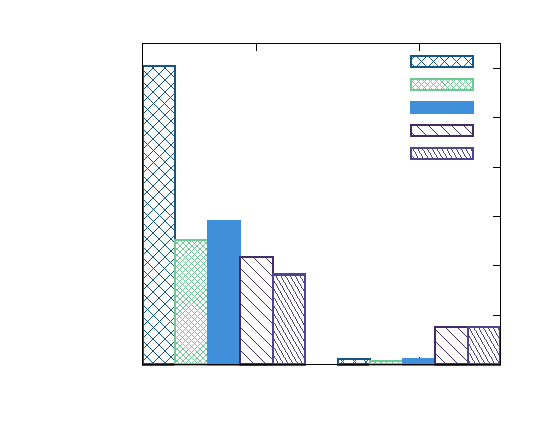
\includegraphics{gsi_throughput}}%
    \gplfronttext
  \end{picture}%
\endgroup

\caption{Single index performance}
\end{figure}



\textbf{Experiment 2:}  We loaded 33 million JSON documents into Couchbase cluster. We created 15 GSI indexes each having 33 million items (total of ~500 million) to drive enough load into the indexer server. This experiment aims at measuring index server throughput.

\begin{table}[h]
\caption{GSI index server performance (items/sec)}
\begin{tabularx}{\linewidth}{|X|l|l|} \hline
Operation&MOI Indexes&Regular Indexes\\ \hline
Create Documents&1,658,031&88,102 \\ \hline
Update Documents&822,680&70,802 \\ \hline
Delete Documents&1,578,316&80,578 \\ \hline
\hline\end{tabularx}
\end{table}

The Table-1 shows that a maximum insertion throughput of 1.65 million items/sec was achieved using Memory Optimized Indexes. This is an order of magnitude improvement compared to the throughput of regular indexes. Document update workload has half the throughput of the document create workload. This is due to the fact that an update translates to a delete and insert operation in the index update engine.

\begin{figure}[h]
% GNUPLOT: LaTeX picture with Postscript
\begingroup
  \makeatletter
  \providecommand\color[2][]{%
    \GenericError{(gnuplot) \space\space\space\@spaces}{%
      Package color not loaded in conjunction with
      terminal option `colourtext'%
    }{See the gnuplot documentation for explanation.%
    }{Either use 'blacktext' in gnuplot or load the package
      color.sty in LaTeX.}%
    \renewcommand\color[2][]{}%
  }%
  \providecommand\includegraphics[2][]{%
    \GenericError{(gnuplot) \space\space\space\@spaces}{%
      Package graphicx or graphics not loaded%
    }{See the gnuplot documentation for explanation.%
    }{The gnuplot epslatex terminal needs graphicx.sty or graphics.sty.}%
    \renewcommand\includegraphics[2][]{}%
  }%
  \providecommand\rotatebox[2]{#2}%
  \@ifundefined{ifGPcolor}{%
    \newif\ifGPcolor
    \GPcolorfalse
  }{}%
  \@ifundefined{ifGPblacktext}{%
    \newif\ifGPblacktext
    \GPblacktexttrue
  }{}%
  % define a \g@addto@macro without @ in the name:
  \let\gplgaddtomacro\g@addto@macro
  % define empty templates for all commands taking text:
  \gdef\gplbacktext{}%
  \gdef\gplfronttext{}%
  \makeatother
  \ifGPblacktext
    % no textcolor at all
    \def\colorrgb#1{}%
    \def\colorgray#1{}%
  \else
    % gray or color?
    \ifGPcolor
      \def\colorrgb#1{\color[rgb]{#1}}%
      \def\colorgray#1{\color[gray]{#1}}%
      \expandafter\def\csname LTw\endcsname{\color{white}}%
      \expandafter\def\csname LTb\endcsname{\color{black}}%
      \expandafter\def\csname LTa\endcsname{\color{black}}%
      \expandafter\def\csname LT0\endcsname{\color[rgb]{1,0,0}}%
      \expandafter\def\csname LT1\endcsname{\color[rgb]{0,1,0}}%
      \expandafter\def\csname LT2\endcsname{\color[rgb]{0,0,1}}%
      \expandafter\def\csname LT3\endcsname{\color[rgb]{1,0,1}}%
      \expandafter\def\csname LT4\endcsname{\color[rgb]{0,1,1}}%
      \expandafter\def\csname LT5\endcsname{\color[rgb]{1,1,0}}%
      \expandafter\def\csname LT6\endcsname{\color[rgb]{0,0,0}}%
      \expandafter\def\csname LT7\endcsname{\color[rgb]{1,0.3,0}}%
      \expandafter\def\csname LT8\endcsname{\color[rgb]{0.5,0.5,0.5}}%
    \else
      % gray
      \def\colorrgb#1{\color{black}}%
      \def\colorgray#1{\color[gray]{#1}}%
      \expandafter\def\csname LTw\endcsname{\color{white}}%
      \expandafter\def\csname LTb\endcsname{\color{black}}%
      \expandafter\def\csname LTa\endcsname{\color{black}}%
      \expandafter\def\csname LT0\endcsname{\color{black}}%
      \expandafter\def\csname LT1\endcsname{\color{black}}%
      \expandafter\def\csname LT2\endcsname{\color{black}}%
      \expandafter\def\csname LT3\endcsname{\color{black}}%
      \expandafter\def\csname LT4\endcsname{\color{black}}%
      \expandafter\def\csname LT5\endcsname{\color{black}}%
      \expandafter\def\csname LT6\endcsname{\color{black}}%
      \expandafter\def\csname LT7\endcsname{\color{black}}%
      \expandafter\def\csname LT8\endcsname{\color{black}}%
    \fi
  \fi
    \setlength{\unitlength}{0.0500bp}%
    \ifx\gptboxheight\undefined%
      \newlength{\gptboxheight}%
      \newlength{\gptboxwidth}%
      \newsavebox{\gptboxtext}%
    \fi%
    \setlength{\fboxrule}{0.5pt}%
    \setlength{\fboxsep}{1pt}%
\begin{picture}(5040.00,3772.00)%
    \gplgaddtomacro\gplbacktext{%
      \csname LTb\endcsname%
      \put(682,704){\makebox(0,0)[r]{\strut{}$0$}}%
      \put(682,1104){\makebox(0,0)[r]{\strut{}$10$}}%
      \put(682,1505){\makebox(0,0)[r]{\strut{}$20$}}%
      \put(682,1905){\makebox(0,0)[r]{\strut{}$30$}}%
      \put(682,2306){\makebox(0,0)[r]{\strut{}$40$}}%
      \put(682,2706){\makebox(0,0)[r]{\strut{}$50$}}%
      \put(682,3107){\makebox(0,0)[r]{\strut{}$60$}}%
      \put(682,3507){\makebox(0,0)[r]{\strut{}$70$}}%
      \put(1293,484){\makebox(0,0){\strut{}MOI}}%
      \put(2729,484){\makebox(0,0){\strut{}Regular}}%
    }%
    \gplgaddtomacro\gplfronttext{%
      \csname LTb\endcsname%
      \put(176,2105){\rotatebox{-270}{\makebox(0,0){\strut{}Throughput (items/sec)}}}%
      \put(2728,154){\makebox(0,0){\strut{}Type of Index}}%
      \csname LTb\endcsname%
      \put(1738,3334){\makebox(0,0)[r]{\strut{}Insert}}%
      \csname LTb\endcsname%
      \put(1738,3114){\makebox(0,0)[r]{\strut{}Update}}%
      \csname LTb\endcsname%
      \put(1738,2894){\makebox(0,0)[r]{\strut{}Delete}}%
    }%
    \gplbacktext
    \put(0,0){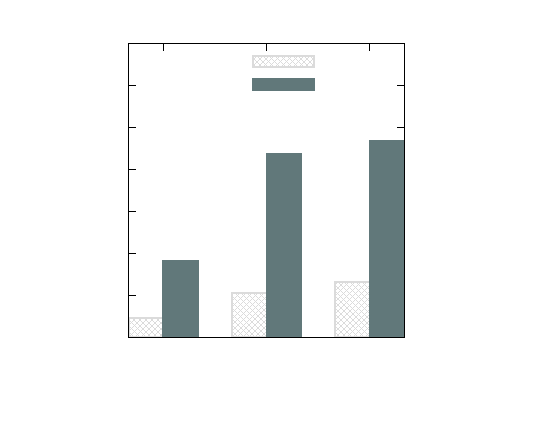
\includegraphics{backuptime}}%
    \gplfronttext
  \end{picture}%
\endgroup

\caption{Index recovery performance}
\end{figure}

\textbf{Experiment 3:} We measured the time taken for index backup and recovery of GSI Memory Optimized Indexes. When this test was performed, there were no background index update or scan in progress. We conducted the experiment with indexes of size 100M, 200M, and 300M items. We observed that the MOI backup performance was limited by the saturation of SSD write throughput while MOI index recovery performance was limited by saturation of CPU cores.

\section{Conclusion}
In this paper, we presented the design of a high performance in-memory index storage engine. We discussed implementation details of lock-free skiplist, Nitro multi-version concurrency control model, garbage collection, backup and recovery, and the performance of Nitro operations. We also proposed a novel algorithm for safe memory reclamation of nodes in the lock-free skiplist. We discussed the design overview of Couchbase global secondary indexes and the details on the implementation of Memory Optimized Indexes using Nitro. Finally, we walked through the performance of Couchbase GSI Memory Optimized Indexes.

 \section{Acknowledgments}
We thank our colleagues Pratap Chakravarthy, Deepkaran Salooja and Prathibha Bisarahalli for the encouragement and support. We also thank Prof. Michael J. Carey for providing the early feedback for the paper. 


\bibliographystyle{abbrv}
\bibliography{memdb.bib}

\end{document}
